\documentclass[longbibliography,slovene,a4paper,12pt]{book}

\usepackage[slovene]{babel}      % slovenski delilni vzorci (!)
\usepackage[utf8]{inputenc}
\usepackage{amsfonts}
\usepackage[T1]{fontenc}
\usepackage[pdftex]{graphicx}
\usepackage{fancyhdr}
\usepackage[sort, numbers]{natbib}
\usepackage{hyperref}
\usepackage{url}
\usepackage[a4paper,inner=3.5cm,outer=2.5cm,top=2.5cm,bottom=2.5cm,pdftex]{geometry}
\usepackage[titletoc,title]{appendix}
\usepackage{epstopdf}
\usepackage{makeidx}

\usepackage[T1]{fontenc}

\usepackage{caption}

\usepackage{pdfpages}
\usepackage{graphicx}
\usepackage{courier}
\usepackage{float}
\usepackage{framed}
\usepackage{hyperref}
\usepackage{amsmath, amssymb}
\usepackage{sidecap}
\usepackage{braket}
\usepackage{subcaption}
\usepackage[normalem]{ulem}
\usepackage[version=3]{mhchem}
\usepackage{lmodern,textcomp}


\newcommand{\HRule}{\rule{\linewidth}{0.5mm}}
\newcommand{\dd}{\text{d}}
\newcommand{\E}{\text{e}}
\newcommand{\I}{\text{i}}
\newcommand{\tr}{\text{ Tr }}
\DeclareMathOperator{\arctg}{arctg}

\pagestyle{headings}
\makeindex


%%
%% Za pisanje sumnikov imamo tri moznosti:
%%   --- vnasamo jih neposredno v kodnem sistemu UTF-8 
%%   --- pisemo jih z latexovim ukazom, ki je namenjen natanko temu,
%%       in sicer kot \v{c}, \v{s}, \v{z}, \v{C}, \v{S}, v{\Z} ali
%%       malo manj pregledno kot \v c, \v s, \v z, \v C, \v S, \v Z,
%%   --- pisemo jih kot "c, "s, "z, "C, "S, "Z), vendar tedaj potrebujemo
%%       spodaj zapisani macro, ki znaku " pripise vlogo `izdelave' sumnika:
%\catcode`\"=\active\def"#1{\v{#1}}
%%       torej \v{S}krjan\v{c}ek == \v Skrjan\v cek == "Skrjan"cek
%% Pozor: narekovaj potem ne smemo vec pisati kot " ampak kot `` in '',
%%       torej: "Skrjan"cek je "civkal ``"ci-"ci-"ci''.

%%
%% Mozni nacini stevilcenja strani:
%%  --- arabske stevilke v celotnem dokumentu, kot je uporabljeno v tej predlogi
%%  --- del strani je lahko stevilcen z rimskimi stevilkami, razen uvoda, osrednjega dela, zakljucka in seznama literature.
%% V vsakem primeru se stevilke na straneh izpisejo sele od kazala naprej.

\def\epsfg#1#2{\epsfig{file=#1.eps,width=#2}}
\def\legendamp#1#2{\vbox{\hsize=#1\caption{\small #2}}}

\setcounter{topnumber}{4}
\setcounter{bottomnumber}{4}
\setcounter{totalnumber}{5}
\renewcommand{\topfraction}{0.99}
\renewcommand{\bottomfraction}{0.99}
\renewcommand{\textfraction}{0.0}
\setlength{\tabcolsep}{10pt}
\renewcommand{\arraystretch}{1.5}

\def\bi#1{\hbox{\boldmath{$#1$}}}
\let\oldvec\vec
\def\vec#1{\mbox{\boldmath$#1$}}
\def\pol{{\textstyle{1\over2}}}
\def\svec#1{\mbox{{\scriptsize \boldmath$#1$}}}

\begin{document}

%%% NASLOVNA STRAN

\pagestyle{empty}
\begin{center}

{\large UNIVERZA V LJUBLJANI\\
FAKULTETA ZA MATEMATIKO IN FIZIKO\\
ODDELEK ZA FIZIKO\\
Fizika in geofizika, fizika kondenzirane snovi\\}


\vspace{4cm}


{\Large Jaka Pišljar\\}

\vspace{10mm}

{\bf \Large Simulacije vodenja svetlobe skozi dvojno-zviti cilinder}\\
\vspace{5mm}
{\large Magistrsko delo}\\




\vfill



{\large MENTOR$\backslash$-ICA: doc. dr., Miha Ravnik\\


\vspace{2cm}
Ljubljana, 2017}

\end{center}

%%% ZAHVALA (NEOBVEZNO)

\cleardoublepage
\mbox{}
\vfill
{\Large \bf Zahvala}
\vspace{1cm}\\
Na tem mestu zapi"site, komu se zahvaljujete za pomoč pri nastanku magistrskega dela.

%%% IZVLECEK

\cleardoublepage
{\Large \bf Izvleček}
\vspace{1cm}\\
Kratek izvle"cek v slovenskem jeziku.\\
\vspace{1cm}\\
{\bf Klju"cne besede:}\\
{\bf PACS:}

%%% ABSTRACT

\cleardoublepage
{\Large \bf Abstract}
\vspace{1cm}\\
Kratek izvle"cek v angle"skem jeziku.
\vspace{1cm}\\
{\bf Keywords:}\\
{\bf PACS:}

%%% KAZALO

\tableofcontents

%%% SEZNAM SLIK (NEOBVEZNO)

\cleardoublepage\phantomsection
\renewcommand\listfigurename{Seznam slik}
\addcontentsline{toc}{chapter}{\listfigurename}
\listoffigures

%%% SEZNAM TABEL (NEOBVEZNO)

\cleardoublepage\phantomsection
\renewcommand\listtablename{Seznam tabel}
\addcontentsline{toc}{chapter}{\listtablename}
\listoftables

\cleardoublepage

%%% OSREDNJI DEL

\pagestyle{fancy}
\fancyhead[CE,RE]{}
\fancyhead[LO,CO]{}
\fancyhead[LE]{\textbf{\nouppercase{\leftmark}}}
\fancyhead[RO]{\textbf{\nouppercase{\rightmark}}}

%\include{Uvod}

%%%%-------------------UVOD-------------------------%%%%%t
\chapter{Uvod}
\label{ch1}

Svetloba je pomembna. Sončna svetloba je energijski vir, ključen za razvoj življenja na Zemlji, dandanes pa se vse več naporov usmerja v razvoj materialov za učinkovito pretvarjanje svetlobe v električno energijo. Praktično v vseh znanstvenih panogah najdemo eksperimente ali eksperimentalne metode, ki izkoriščajo lastnosti svetlobe, dober primer je potrditev obstoja gravitacijskih valov, ki so jih zaznali s pomočjo 4 km dolgega interferometra\cite{abbott}. Na kemijskem, biološkem ter medicinskem področju je ključen razvoj optične mikroskopije, ki omogoča opazovanje pod difrakcijsko limito \cite{klar} ter novih načinov slikanja, ki na primer omogočajo slikanje ultrahitrih procesov\cite{mikami}. V industriji lasersko svetlobo že desetletja izkoriščajo za obdelavo materialov: poliranje, rezanje, varjenje \emph{itn.} Verjetno najbolj razširjena uporaba svetlobe pa je za hitro \emph{komunikacijo} po celem svetu prek optičnih vlaken\cite{willner}. \\

Veliko raziskav na področju fotonike in optike je usmerjene tudi v materiale z zanimivimi ali neobičajnimi optičnimi lastnostnmi, kot so (elektromagnetni) \emph{metamateriali}. To so umetno pripravljeni materiali, ki jih v naravi ne najdemo, pri njihovem nastanku pa gre za krojenje periodičnih struktur iz običajnih materialov, na razdaljah običajno veliko krajših od valovne dolžine svetlobe.  Največ zanimanja so bili deležni metamateriali z negativnim lomnim količnikom\cite{shelby,soukolis} ter takšni, ki omogočajo maskiranje pred elekromagnetnimi valovi\cite{pendry,ergin}.\\

Tehnološko čedalje bolj zanimiva stvar na področju fotonike pa so tudi \emph{fotonska vezja}. Sestavlja jih serija optičnih vlaken prepletenih z optičnimi ter občasno tudi elektronskimi elementi s katerimi izvajamo logične operacije\cite{siliconphotonics}. Zaradi potencialno hitrejšega pretoka informacij v in med vezji računalniški velikani kot sta IBM ter Intel veliko vlagata v raziskave teh vezij na osnovi siliciija\cite{siliconphotonicsintel}. K razvoju teh vezij je pripomogel razvoj različnih optičnih elementov, ki jih sicer poznamo iz elektronskih vezij kot so fotonska stikala\cite{bose}, logična vrata\cite{espinosa} ter optični tranzistorji\cite{chen}.\\

Tekoči kristali so že desetletja osnova za delovanje zaslonov raznovrstnih elektronskih naprav, osnovanih na principu preurejanja tekočega kristala ob odzivu na zunanje električno polje, ki pomeni spremembo optičnih lastnosti prepuščene svetlobe\cite{yeh}. V fiziki tekočih kristalov pa se zadnja leta pozornost vse bolj usmerja k uporabi tekočih kristalov v fotoniki in fotonskih vezjih\cite{musevic}. Zanimivo področje so tekočekristalni laserji, ki temeljijo na osnovi periodičnosti tekočega kristala in obstoju vrzeli, prepovedanega pasu v kiralnih tekočih kristalih, ki preprečuje širjenje svetlobe določenih valovnih dolžin\cite{coles2}. 

%%%%-------------------TEORIJA-------------------------%%%%%
\chapter{Teoretični uvod}
%%%%-------------------OPIS ELEKTROMAGNETNEGA VALOVANJA-------------------------%%%%%
\section{Opis elektromagnetnega valovanja}
Elektromagnetno valovanje opišemo s setom štirih Maxwellovih enačb, ki jih v snovi zapišemo kot
\begin{subequations}
\label{maxwell}
\begin{align}
\nabla \cdot \mathbf{D} &= \rho_e & \nabla \times \mathbf{E} &= -\frac{\partial \mathbf{B}}{\partial t}\label{a}\\
\nabla \cdot \mathbf{B} &= 0   & \nabla \times \mathbf{H} &= \mathbf{j} +  \frac{\partial \mathbf{D}}{\partial t} \label{b},
\end{align}
\end{subequations}
kjer sta $\mathbf{E}$ in $\mathbf{H}$ električno in magnetno polje svetlobe, $\mathbf{D}$ in $\mathbf{B}$ pa njuni gostoti. $\rho_e$ in $\mathbf{j}$ sta električni naboj in gostota električnega toka v snovi, in predstavljata izvora elektromagnetnih polj\cite{podgornik}. Ker nas bodo zanimali zgolj primeri ko v snovi ni izvorov bo $\rho_e = \mathbf{j} = 0$. Polji in njuni gostoti v snovi med seboj povezujeta \emph{konstituitivni relaciji}, ki jih v \emph{linearnih materialih} zapišemo kot
\begin{align}
\mathbf{D} = \varepsilon \varepsilon_0 \mathbf{E} \quad \quad \mathbf{B} = \frac{1}{\mu \mu_0} \mathbf{H},
\label{constituitive}
\end{align}
kjer sta $\varepsilon_0$ ter $\mu_0$ \emph{električna permitivnost} ter \emph{magnetna permeabilnost} vakuuma, $\varepsilon$ in $\mu$ pa permitivnost in permeabilnost snovi, parametra ki sta v splošnem krajevno, časovno, v disperzivnih materialih tudi frekvenčno odvisna, ter opisujeta odziv snovi na električno oziroma magnetno polje. Tipično je v tekočih kristalih odziv na magnetno polje zanemarljiv in $\mu = 1$. Kot pa bomo spoznali, je ključna lastnost, ki loči tekoče kristale od tekočin njihova \emph{anizotropna faza}, kjer je dielektrična permitivnost (oziroma krajše \emph{dielektričnost}) $\varepsilon$ ne le funkcija koordinat, pač pa je odvisna tudi od lokalne smeri $\mathbf{E}$: to je \emph{tenzorska} količina, ki jo v splošnem opišemo s $3 \times 3$ matriko s šestimi neodvisnimi komponentami\cite{podgornik}. \\

Skupaj s konstiutivnima relacijama so enačbe \ref{maxwell} medsebojno sklopljene, zato jih lahko še nekoliko preoblikujemo, če  $\nabla \times$ pomnožimo z enačbo (\ref{maxwell}) ter upoštevamo vektorsko relacijo
\begin{equation}
\nabla \times \nabla \times \mathbf{E} = \nabla(\mathbf{\nabla} \cdot \mathbf{E}) - \nabla^2 \mathbf{E}.
\end{equation}
Ob prejšnjih predpostavkah brezizvornega $\rho_e = \mathbf{j} = 0$ in $\mu = 1$ dobimo
\begin{equation}
\nabla(\nabla \cdot \mathbf{E})  - \nabla^2 \mathbf{E} = - \frac{\partial}{\partial t} \left (\nabla \times \frac{\mathbf{H}}{\mu_0} \right ).
 \end{equation} 
Sedaj na desni strani upoštevamo relacijo med $\mathbf{D}$ in $\mathbf{E}$, na desni pa moramo biti previdni, saj je v nehomogenih snoveh $\varepsilon = \varepsilon(\mathbf{r})$ in torej iz enačbe 11a sledi
 
 \begin{equation}
 \nabla \cdot \mathbf{D} = \nabla \cdot (\varepsilon(\mathbf{r}) \varepsilon_0 \mathbf{E}) = \varepsilon_0 \left ( \nabla \varepsilon \cdot \mathbf{E}  + \varepsilon \nabla \cdot \mathbf{E} \right ) = 0,
 \end{equation}
 kar da zvezo 
 \begin{equation}
 \nabla \cdot \mathbf{E} = -\left (\frac{1}{\varepsilon} \right ) \nabla \varepsilon \cdot \mathbf{E}.
 \end{equation}
 
 Sedaj lahko iz enačbe (13) dobimo enačbo, ki vsebuje zgolj $\mathbf{E}$
 
 \begin{equation}
 \nabla^2 \mathbf{E} + \nabla \left(\frac{1}{\varepsilon} \nabla \varepsilon \cdot \mathbf{E}\right) - \mu_0 \varepsilon_0 \varepsilon \frac{\partial^2\mathbf{E}}{\partial t^2} = 0.
 \label{anisotropicwaveequation}
 \end{equation}
 
 Na tem mestu napravimo prvi približek, ko predpostavimo, da se funkcija $\varepsilon(\mathbf{r})$ spreminja počasi na razdaljah primerljivih z valovno dolžino svetlobe.\footnote{V nematskih profilh s katerimi imamo opravka, se, spremembe velikosti nekaj odstotkov $n(\mathbf{r}) = \sqrt{\varepsilon(\mathbf{r})}$ tipično zgodijo na razdaljah nekaj mikronov, tipična  valovna dolžina svetlobe pa je $\lambda = 390$nm.} Takrat je drugi člen v enačbi (\ref{anisotropicwaveequation}) zanemarljiv v primerjavi s prvim in lahko zapišemo valovno enačbo
 
 \begin{equation}
 \nabla^2 \mathbf{E} - \frac{1}{c^2(\mathbf{r})} \frac{\partial^2 \mathbf{E}}{\partial t^2} = 0,
  \label{Ewaveequation}
 \end{equation}
 
 kjer je $c(\mathbf{r}) = 1/\sqrt{\mu_0 \varepsilon_0 \varepsilon} = c_0/n(\mathbf{r})$ lokalna \emph{hitrost svetlobe} in $n(\mathbf{r}) = \sqrt{\varepsilon(\mathbf{r})}$ \emph{lomni količnik} na mestu $\mathbf{r}$ \cite{saleh}.\\
 
 Zanimajo nas rešitve valovne enačbe za $\mathbf{E}$, ki imajo konstantno frekvenco $\omega$ in se širijo v določeni smeri. Takšne \emph{monokromatske} elektromagnetne valove opisujeta naslednji krajevno-časovni odvisnosti svetlobnih polj 
 
 \begin{align}
 &\mathbf{E} (\mathbf{r}, t) = \mathbf{E}(\mathbf{r}) \E^{\I \omega t} \label{Efield}\\
 &\mathbf{B} (\mathbf{r}, t) = \mathbf{B}(\mathbf{r}) \E^{\I \omega t} \label{Bfield}, 
 \end{align}
 
kjer je $\omega = 2\pi \nu$ krožna frekvenca svetlobe \cite{saleh}.

%-----------ravni valovi in tenzor dielektričnosti----------%
\section{Ravni valovi in tenzor dielektrične permitivnosti}

Ena izmed najenostavnejših rešitev valovne enačbe so ravni valovi. V tem primeru kompleksni vektor električnega polja $\mathbf{E(\mathbf{r})}$, ki nastopa v enačbi (\ref{Efield}) zapišemo kot
\begin{equation}
\mathbf{E} (\mathbf{r}) = \mathbf{E}_0 \E^{-\I\mathbf{k} \cdot \mathbf{r}},
\end{equation}
kjer je $\mathbf{E}_0$ konstantni vektor amplitude električnega polja v ravnem valu, $\mathbf{k}$ pa valovni vektor z amplitudo $k = |\mathbf{k}|$. Podobno velja za magnetno polje \ref{Bfield}. V tem primeru velja $\nabla \times \mathbf{E} = \I \mathbf{k}\times \mathbf{E}$ in $\partial \mathbf{E}/\partial t=-\I \omega \mathbf{E}$. Če slednje uporabimo za zapis vektorske valovne enačbe za $\mathbf{E}$ dobimo

\begin{equation}
\mathbf{k} \times (\mathbf{k} \times \mathbf{E}) = -\omega^2 \mu_0 \mathbf{D}
\end{equation}
oziroma ob uporabi konstitutivne relacije $\mathbf{D} = \varepsilon \mathbf{E}$ 
\begin{equation}
\mathbf{k} \times (\mathbf{k} \times \mathbf{E}) + \omega^2 \mu_0 \varepsilon \mathbf{E} = 0.
\end{equation}
To je vektorska enačba za $\mathbf{E}$ in se prevede na tri linearne enačbe, ki jim morajo zadostiti komponente $\mathbf{E} = (E_1,E_2,E_3)$, kar lahko v matrični obliki zapišemo kot
\begin{equation}
\begin{pmatrix} \varepsilon_{11}k_o^2-k_2^2-k3^2 & k_1k_2 & k_1k_3 \\
				k_2k_1 &  \varepsilon_{22}k_o^2-k_1^2-k_3^2 & k_2k_3\\
				k_3k_1 & k_3k_2 &  \varepsilon_{33}k_o^2-k_1^2-k_2^2	
	   \end{pmatrix} \cdot \begin{pmatrix}E_1 \\ E_2 \\ E_3 \end{pmatrix}= \begin{pmatrix}0 \\ 0 \\ 0 \end{pmatrix}.
\label{uniaxialQ}
\end{equation}

Tu je $k_o = \omega/c_0$ in $\varepsilon_{ii}$ diagonalne vrednosti $\varepsilon_{ij}$ zapisanega v lastnem koordinatnem sistemu. Nadalje velja, da je lomni količnik $n_i = \sqrt{\varepsilon_{ii}}$. Če izračunamo determinanto gornje matrike dobimo rezultat, ki da $\omega = \omega(k_1,k_2,k_3)$ in predstavlja dve centrosimetrični površini v $k$-prostoru. Površini sta določeni z vrednostmi $n_i$ in njuni presečišči določajo optične osi v materialu. To si oglejmo na primeru bolj enostavnega enoosnega kristala, kjer naj velja $n_1=n_2=n_o$ in $n_3 = n_e$. Tedaj pogoj za ničelno determinanto razpade na
\begin{equation}
(k^2-n_o^2k_o^2)\left(\frac{k_1^2+k_2^2}{n_e^2} + \frac{k_3^2}{n_o^2} -k_o^2\right ) =0.
\end{equation}
Enačba predstavlja dve površini: levi faktor predstavlja sfero z $k=n_ok_o$ desni pa elipsoid z dvema polosema $n_o$ in $n_e$. Del površin in njuno presečišče, ki sedaj določa eno samo optično os (smer $z$), je prikazano na Sliki  \ref{fig:uniaxialsurface3d}. Če privzamemo, da $\mathbf{k}$ vektor svetlobe leži v ravnini $xz$ ter oklepa kot $\theta$ z optično osjo presečišče tega vekotorja z obema krivuljama določa \emph{lastne načine} oziroma dovoljene velikosti valovnega števila $k$ v tem materialu: redni in izredni način\cite{saleh}. To je prikazano na Sliki \ref{fig:uniaxialsurface2d}.

\begin{figure}[h!]
	\centering
	\begin{subfigure}[b]{0.45\textwidth}
	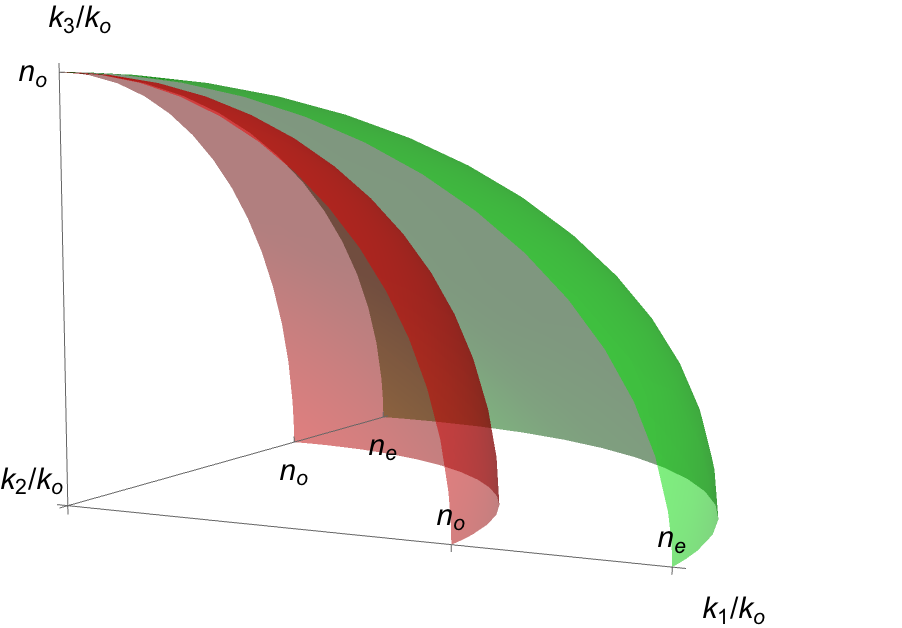
\includegraphics[width=\textwidth]{slike/uniaxial_k_surfaces.png}
	\phantomcaption
	\label{fig:uniaxialsurface3d}
	\end{subfigure}
	\begin{subfigure}[b]{0.45\textwidth}
	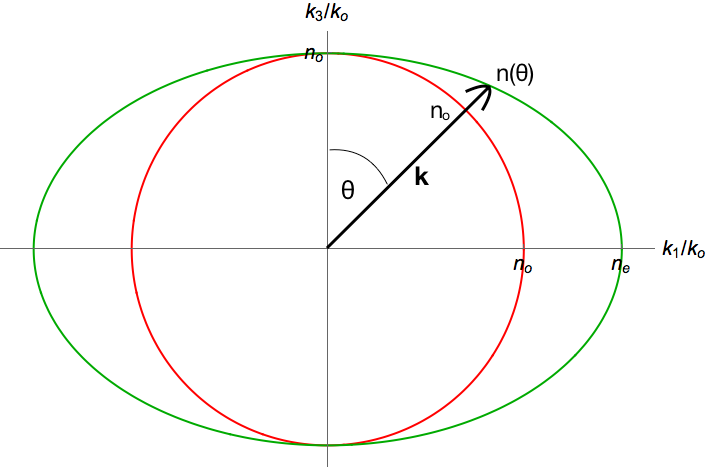
\includegraphics[width=\textwidth]{slike/uniaxial_k_surfaces_2d_edited.png}
	\phantomcaption
	\label{fig:uniaxialsurface2d}
	\end{subfigure}
	\caption{\emph{\textbf{a.)} Površini konstantnega $\mathbf{k}$ v primeru običajnega in neobičajnega lomnega količnika. \textbf{b.)} Elipsi v primeru, ko ima $\mathbf{k}$ le $x$ in $z$ neničelni komponenti. Lomna količnika lastnih načinov sta določena s presečiščem vektorja $\mathbf{k}$ z obema elipsama -- $n_o$ in $n(\theta)$, kjer je $\theta$ označeni kot med optično osjo  ter vektorjem $\mathbf{k}$.}}
\end{figure} 

Iz Slike \ref{fig:uniaxialsurface2d} vidimo, da ima redni način ne glede na kot $\theta$ valovno število $k=n_o k_o$ medtem ko ima izredni način $k=n(\theta)n_o$, kjer je 
\begin{equation}
\frac{1}{n^2(\theta)} = \frac{\cos^2 \theta}{n_o^2} + \frac{\sin^2 \theta}{n_e^2}.
\label{extraordinaryn}
\end{equation}
Vsak lastni način določa tudi njemu lastno polarizacijo! Iz konstrukcije namreč lahko sklepamo, da ima svetloba, ki se razširja vzdolž lastne osi $z$ ne glede na kot polariziacije lomni količnik $n_o$. Če se svetloba širi v vzdolž osi $x$ je polarizirana v ravnini $yz$. Tam ima lomni količnik $n_o$, če je polarizirana vzdolž osi $y$ ali $n_e$, če je polarizirana v smeri optične osi: to sta lastni polarizaciji za redni in izredni način v tem primeru. V primeru, ko pa ima polarizacija poljubno smer v ravnini $yz$ takšna polarizacija razpade na polarizaciji lastnih načinov\cite{saleh}. Ti dve se zaradi razlike v lomnih količnikih gibljeta z različnima hitrostma, zato sta po prepotovani razdalji $d$ lastni komponenti medsebojno fazno zamaknjeni za 
\begin{equation}
\varphi = \varphi_o - \varphi_e = k_o(n_o - n_e)d.
\end{equation}
Splošneje, v primeru, ko se svetloba giblje v poljubni smeri, ki oklepa kot $\theta$ z optično osjo poljubna polarizacija v ravnini pravokotni na to smer razpade na lastni polarizaciji, ki občutita lomna količnika $n_o$ in $n(\theta)$ in fazni zamik je
\begin{equation}
\varphi = \varphi_o - \varphi_e = k_o(n_o - n(\theta))d.
\end{equation}

%%%----------------------SVETLOBNI SNOPI----------------%

\section{Svetlobni snopi}
Zgoraj opisani ravni valovi, so zgolj matematična rešitev v kateri se valovne fronte raztezajo v neskončnost in se s časom ne spreminjajo. Tega v naravi ne opazimo, vendar pa koncept vseeno dobro služi pri opisu nekaterih lastnosti svetlobe, na primer dvolomnosti, kot smo pokazali v prejšnjem poglavju. Rešitve valovne enačbe, ki so za nas bolj zanimive pa so prostorsko omejene in s prepotovano razdaljo ali s časom spreminjajo svojo obliko. To so \emph{svetlobni snopi}, ki jih ponavadi povezujemo z laserji. Osnovni snop, ki ga spoznamo pri študiju laserjev je \emph{Gaussov snop}, ki ga matematično opišemo tako, da predpostavimo smiselen nastavek snopa svetlobe, ki se razširja vzdolž osi $z$ ampak je prostorsko omejen v transverzalni ravnini $xy$ v kateri leži tudi njegova polarizacija

\begin{equation}
\mathbf{E}(\mathbf{r}, t) = E_0 \mathbf{e_\perp}U(\mathbf{r}) \E^{\I kz - \I \omega t},
\label{gaussianansatz}
\end{equation}

kjer je $E_0$ konstantna amplituda, $U(\mathbf{r})$ pa amplitudna funkcija odvisna od vseh treh koordinat, $\mathbf{e_\perp}$ pa enotski vektor v $xy$ ravnini. Ob predpostavki, da se amplituda $U$ spreminja počasi vzdolž koordinate $z$ \footnote{V izpeljavi predpostavimo, da $\frac{\partial^2 U}{\partial z^2} \ll \frac{\partial U}{\partial z}$ in tako $\nabla^2 \rightarrow \nabla_T^2$.} vstavimo nastavek v valovno enačbo za $\mathbf{E}$ dobimo \emph{skalarno} obosno Helmholtzevo enačbo za amplitudo $U(\mathbf{r})$

\begin{equation}
\nabla_T^2 U + 2\I k \frac{\partial U}{\partial z} = 0.
\label{helmholtzequation}
\end{equation}

Osnovna rešitev te enačbe v kartezični geometriji je Gaussov snop, z amplitudo

\begin{equation}
U(\mathbf{r}) = \frac{w_0}{w(z)} \exp \left ( -\frac{\rho^2}{w(z)^2} \right ) \exp \left (-\I k \frac{\rho^2}{2R(z)} \right ) \exp(\I \eta(z)),
\label{gaussianamplitude}
\end{equation}

kjer je $w_0$ polmer v grlu, najbolj ozkem delu snopa, $w(z)$ polmer snopa na koordinati $z$, z izhodiščem v grlu, $\rho^2 = x^2 +y^2$, $R(z)$ krivinski radij valovnih front na mestu $z$, $\eta(z) = \arctg (z/z_0)$ pa t.i. Gouyeva faza, ki predstavlja od koordinate $z$ odvisni dodatek k običajni fazi $\I kz$ ravnih valov.. Struktura rešitve \ref{gaussianamplitude} je produkt treh eksponentnih funkcij, ki po vrsti opisujejo Gaussovsko amplitudo žarka v trasnverzalni smeri, zakrivljenost valovnih front ter dodatni fazni zamik v Gaussovem snopu\cite{saleh}. Intenzitetni profil Gaussovega snopa za nek $z$ je prikazan na Sliki \ref{fig:gaussianbeam} njegov profil vzdolž osi $z$ pa na Sliki \ref{fig:gaussianbeamprofile}.
\begin{figure}[h!]
	\centering
	\begin{subfigure}[b]{0.35\textwidth}
	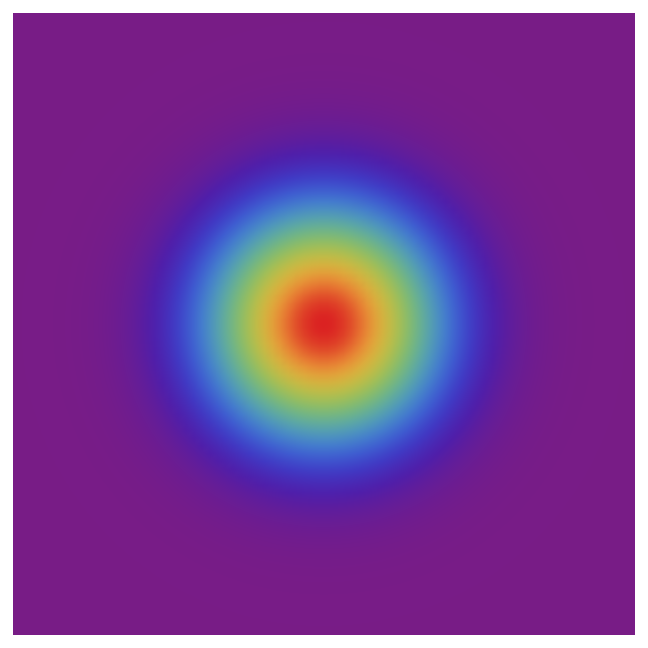
\includegraphics[width=\textwidth]{slike/lg_00.png}
	\phantomcaption
	\label{fig:gaussianbeam}
	\end{subfigure}
	\quad
	\begin{subfigure}[b]{0.45\textwidth}
	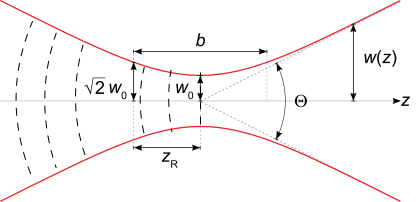
\includegraphics[width=\textwidth]{slike/gaussian_beam_profile_edited.png}
	\phantomcaption
	\label{fig:gaussianbeamprofile}
	\end{subfigure}
	\caption{\emph{Intenzitetni profile Gaussovega snopa ter njegov vzdolžni profil z označenimi ključnimi parametri Gaussovih snopov kot so širina grla $w_0$, Rayleigheva razdalja $z_R$ ter divergenca snopa $\Theta$. S črtkanimi črtami je prikazana tudi zakrivljenost valovnih front.}}
\end{figure} 

Poleg Gaussovega snopa svetlobe, moramo omeniti še rešitve enačbe \ref{helmholtzequation} v cilindrični geometriji, saj bodo pomembne v nadaljevanju. Ko za izračun uporabimo cilindrično verzijo $\nabla_T^2$ dobimo t.i. \emph{Laguerre-Gaussov snop}, rešitev za $U$ odvisno od radija $\rho$, azimutalnega kota $\phi$ ter $z$

\begin{equation}
U(\rho, \phi, z) = \left( \frac{\rho}{w(z)} \right )^{|\ell|} \frac{w_0}{w(z)}  L_p^\ell \left (2\frac{\rho^2}{w(z)^2} \right )  \exp \left ( -\frac{\rho^2}{w(z)^2} - \I k\frac{\rho^2}{2R(z)} - \I \eta_{p\ell} (z) \right ) \exp [ -\I \ell \phi].
\label{laguerregaussianamplitude}
\end{equation}

Tu so $L_p^\ell$ pridruženi Laguerrovi polinomi, $\eta_{p\ell} = (2p + \ell + 1) \arctg(z/z_0)$ pa posplošena Gouyeja faza. Izraz \ref{laguerregaussianamplitude} je zapleten, zato omenimo le nekaj pomembnih lastnosti. Različni redi rešitev so opisani z različnima vrednostima $\ell$ in $p$.Vrednosti $p$ določajo koliko ničel ima Laguerre-Gaussov polinom in zato tudi koliko intenzitetnih minimumov bo imel tak žarek. $\ell=p=0$ pa vrne izraz \ref{faussianamplitude}.Ko $\ell \neq 0$ ima zaradi prvega faktorja intenzitetni profil takega žarka ničelno intenziteto pri $\rho = 0$. To je prikazano na Slikah \ref{fig:lg_01beam} ter \ref{fig:lg_21beam}, kjer sta prikazana dva intezitetna profila Laguerre-Gaussovih snopov.
\begin{figure}[h!]
	\centering
	\begin{subfigure}[b]{0.31\textwidth}
	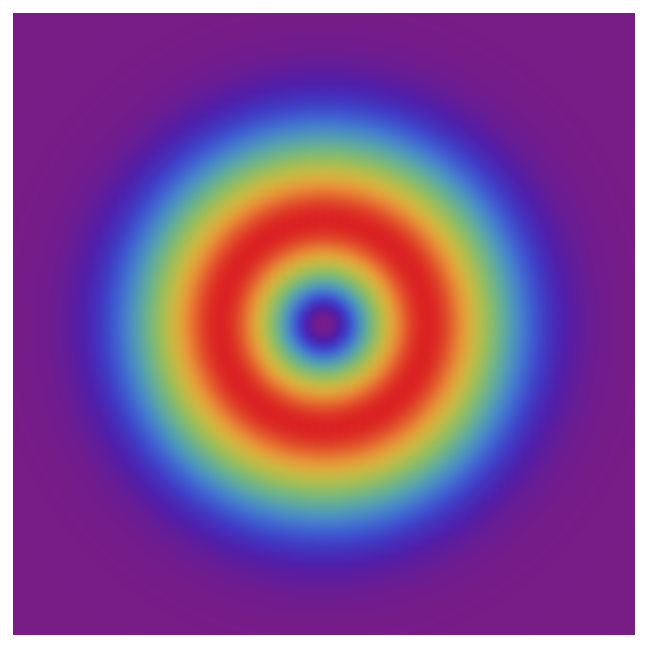
\includegraphics[width=\textwidth]{slike/lg_01.png}
	\phantomcaption
	\label{fig:lg_01beam}
	\end{subfigure}
	\begin{subfigure}[b]{0.31\textwidth}
	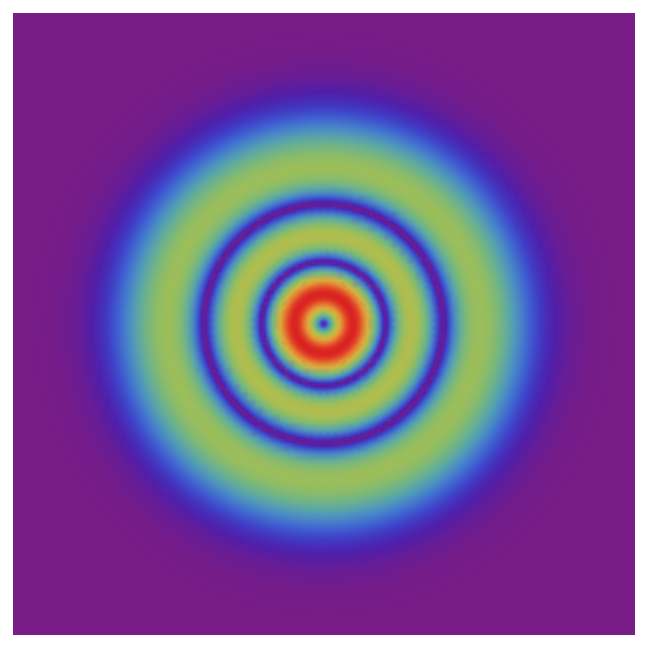
\includegraphics[width=\textwidth]{slike/lg_21.png}
	\phantomcaption
	\label{fig:lg_21beam}
	\end{subfigure}
	\begin{subfigure}[b]{0.35\textwidth}
	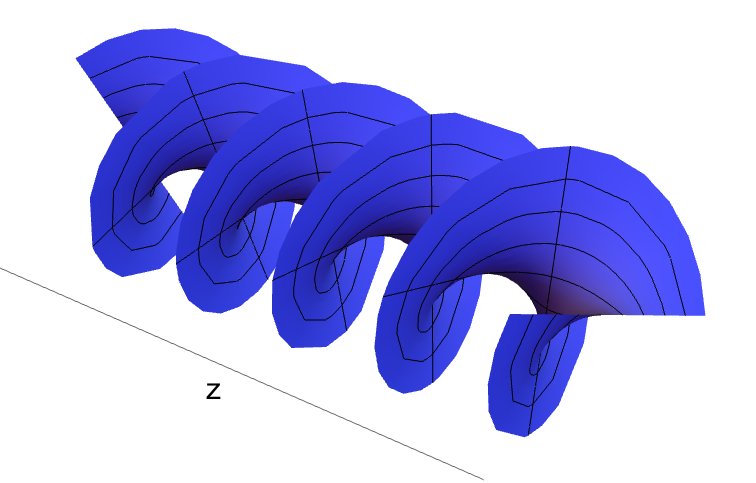
\includegraphics[width=\textwidth]{slike/helical_beam.png}
	\phantomcaption
	\label{fig:lg_01azimuthalbeam}
	\end{subfigure}
	\caption{\emph{Intenzitetni profila dveh Laguerre-Gaussovih snopov z ($p = 0$, $l=1$) ter ($p=2$, $l=1$).}}
\end{figure} 
Zadnji faktor v izrazu (\ref{laguerregaussianamplitude}) je t.i. vrtinčna faza (\emph{vortex phase}) $\E^{\I \ell \phi}$, ki pomeni, da se \emph{faza} električnega polja linearno povečuje z azimutalnim kotom $\phi = \arctg(y/x)$, $\ell$ pa določa za kakšen večkratnik $2\pi$ se faza spremeni ob enem obratu. To pomeni, da se valovna fronta žarka spiralno suče okoli osi $z$, kar daje Laguerre-Gaussovim snopom vrtilno količino\cite{saleh}.\\

V gornjem nastavku \ref{gaussianansatz} smo predpostavili \emph{homogeno} polarizacijo, pravokotno na smer žarka, kar je enačbe prevedlo na skalarno obliko. Nas pa bodo zanimale drugačne rešitve, takšne kjer dovolimo, da se polarizacija spreminja s koordinatama $x$ in $y$.

%%%----------------------vektorski snopi----------------%
\subsection{Vektorski snopi svetlobe}

V cilindrični geometriji, lahko poskušamo najti rešitve \emph{vektorske} valovne enačbe

\begin{equation}
\nabla \times \nabla \times \mathbf{E} - k^2 \mathbf{E} = 0
\end{equation}

z nastavkom \emph{azimutalne} polarizacije 

\begin{equation}
\mathbf{E} (\rho,z) = U(\rho, z) \E^{\I (kz-\omega t)} \mathbf{e}_\phi,
\end{equation}
kjer ima polarizacija v vsaki točki $(\rho, \phi, z)$ azimutalno usmeritev $\mathbf{e}_\phi \perp \mathbf{e}_{r}$. V tem primeru, ima magnetno polje svetlobe $\mathbf{H}$ v vsaki točki radialno smer. Obratna rešitev je t.i. \emph{radialna polarizacija}, kjer električno polje povsod kaže radialno navzven v smeri $\mathbf{e}_{r}$. Že iz nastavka sledi, da v sredini takšnega snopa polarizacija nima definirane smeri zato ima tudi ta profil tam intenzitetno ničlo. Izkaže se, da je amplituda $U(\rho, \phi, z)$ takšnih žarkov enaka Laguerre-Gaussovi \ref{laguerregaussianamplitude} z $\ell > 0$, a v osnovi brez dodanega vrtičnega faktorja\cite{zhan}. Primera takšnih dveh rešitev sta prikazana na Sliki \ref{fig:lg_01radialbeam} ter \ref{fig:lg_01azimuthalbeam}.
\begin{figure}[h!]
	\centering
	\begin{subfigure}[b]{0.35\textwidth}
	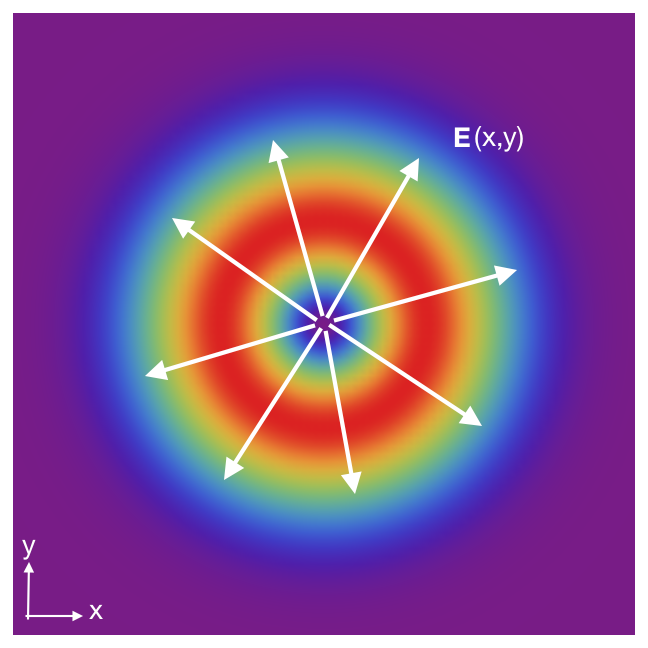
\includegraphics[width=\textwidth]{slike/lg_01_radial.png}
	\phantomcaption
	\label{fig:lg_01radialbeam}
	\end{subfigure}
	\quad
	\begin{subfigure}[b]{0.35\textwidth}
	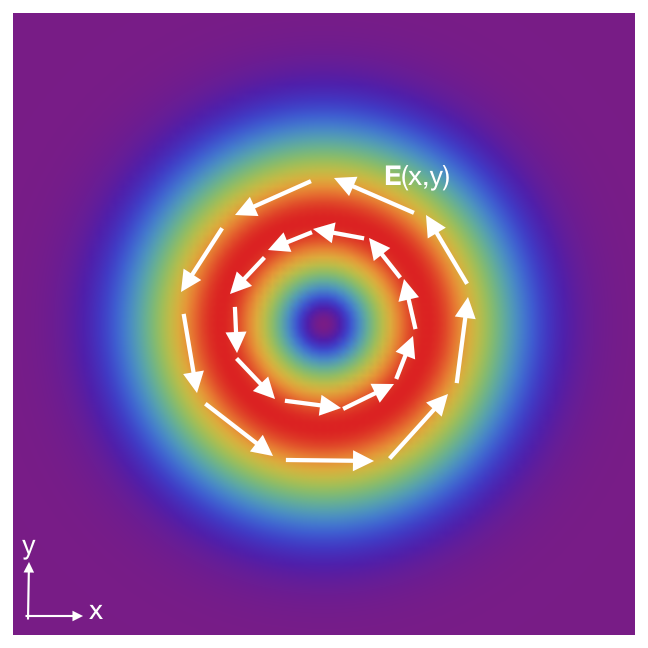
\includegraphics[width=\textwidth]{slike/lg_01_azimuthal.png}
	\phantomcaption
	\label{fig:lg_01azimuthalbeam}
	\end{subfigure}
	\caption{\emph{Vektorska snopa svetlobe z radialno in azimutalno polarizacijo in intenzitetnim profilom osnovnega Laguerre-Gaussovega snopa ($p=0$, $\ell = 1$).}}
\end{figure}

Opisane snope, kjer se smer polarizacije spreminja v odvisnosti od transverzalnih koordinat $x$ in $y$, oziroma $\rho$ ter $\phi$ imenujemo \emph{vektorski snopi svetlobe}. Ena izmed zanimivih lastnosti radialno polariziranega snopa je, da ga je z lečo z veliko numerično aperturo mogoče zbrati v precej manjši presek ($0.16\lambda^2$) pravilne oblike kot pri linearno polariziranih snopih ($0.26\lambda^2$), kjer se pri močnem fokusiranju žarek popači in trči ob teoretično limito. Ta lastnost je posledica dejstva, da se pri močnem fokusiranju pojavijo neničelne \emph{longitudinalne} komponente električnega polja $E_z$, vzporednje z smerjo širjenja, ki pri linearno polariziranih snopih niso radialno simetrične pri radialno polariziranih vektorskih snopih pa so\cite{dorn}.\\

Zmožnost močnejšega fokusiranja vektorskih snopov je bila izkoriščena pri lovljenju delcev\cite{dorn}, laserskem rezanju\cite{niziev} ter optični mikroskopiji\cite{youngworth}. Večinoma jih generirajo iz linearno polariziranih snopov s pomočjo stožičastih Brewsterjevih prizem\cite{kozawa}, posebnih optičnih vlaken, ki dovoljujejo le nekaj lastnih načinov\cite{volpe} ter v zadnjem času vse bolj s pomočjo tekoče kristalnih faznih modulatorjev\cite{ko}. Simulacije iz leta 2014 opravljene z metodo, ki jo bomo uporabili tudi v tem delu pa kažejo, da je mogoče vektorske snope svetlobe generirati tudi na nematskih defektnih linijah\cite{cancula2}.


%------------------------TEKOČI KRISTALI------------------------%

\section{Tekoči kristali}

Z imenom \emph{tekoči kristali} poimenujemo snovi pri katerih v nekem temperaturnem območju obstaja vmesna faza med tekočino in trdno snovjo. Takšna faza ima nekatere lastnosti ki so značilne za tekočo fazo, kot je na primer ta, da tečejo in imajo viskoznost ter druge značilne za trdno snov na primer anizotropijo, orientacijsko urejenost molekul v primeru \emph{nematikov} in \emph{holesterikov} ali prostorski red dolgega dosega v eni oziroma dveh dimenzijah v primeru, holesterikov, \emph{smektikov} in \emph{stebričnih faz}. Shematska primerjava nekaterih tekočekristalnih faz je prikazana na Sliki \ref{fig:liquidcrystaltypes}.\\

\begin{figure}[h!]
	\centering
	\begin{subfigure}[b]{0.9\textwidth}
	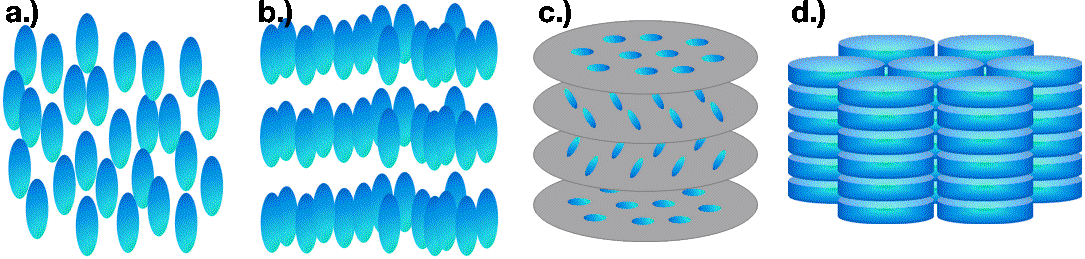
\includegraphics[width=\textwidth]{slike/lc.png}
	\end{subfigure}
	\caption{\emph{Nematska, smektična, holesterična ter stebričasta faza tekočih kristalov. Pri nematski fazi je prisoten zgolj orientacijski red molekul medtem ko pri ostalih fazah opazimo tudi prostorski red v eni (\textbf{b.)}, \textbf{c.)}) ali dveh dimenzijah (\textbf{c.)}). Vir slike:\cite{liquidcrystaltypes}}}
	\label{fig:liquidcrystaltypes}
\end{figure}
Glede na to na kakšen način pridobimo tekočekristalno fazo, ločimo \emph{termotropne} in \emph{liotropne} tekoče kristale. Pri prvih je ključen parameter s katerim določamo fazo snovi \emph{temperatura} pri drugih pa \emph{koncentracija} molekul, ki tvorijo tekoči kristal. V katero izmed teh dveh skupin nek tekoči kristal spada določa struktura osnovnih gradnikov -- za termotropne tekoče kristale so značilne paličaste ali diskaste organske molekule tipičnih dimenzij $300 \times 20$Å,  medtem ko gre pri liotropnih za daljše paličaste molekule velikosti nekaj 10$\mu m$ v substratu. V tem delu se bomo ukvarjali zgolj s termotropnimi nematiki, ki doživijo fazni prehod iz neurejene izotropne v delno urejeno nematsko fazo pri karakteristični temperaturi $T_{NI}$. Za lastnosti termotropnih tekočih kristalov sta ključni kemijska struktura in oblika organskih molekul, ki jih sestavljajo\cite{degennes}. 

%--------------------nematiki-------------------%
\subsection{Nematiki}
 
Nematsko fazo tekočega kristala od izotropne tekočine loči orientacijska urejenost molekul na razdaljah, ki so velike v primerjavi z dimenzijo molekul. Medtem ko so v izotropni fazi molekule usmerjene povsem naključno in neodvisno od drugih molekul, lahko v nematikih govorimo o preferirani (lokalni) usmeritvi molekul, ki jo imenujemo \emph{direktor} matematično pa opišemo z enotskim vektorjem $\mathbf{n}(\mathbf{r})$, definiran kot ansambelsko povprečje orientacij posameznih molekul $\mathbf{s}$ v izbranem volumnu. Zaradi simetrije v nematiku velja enakost $\mathbf{n} = -\mathbf{n}$. Nematski red v običajnih nematikih opišemo s t.i. \emph{stopnjo urejenosti} $S$, ki je mera za termične fluktuacije smeri posameznih molekul $\mathbf{s}$ od smeri direktorja $\mathbf{n}$ in je definirana kot 

\begin{equation}
S = \langle P_2(\mathbf{s} \cdot \mathbf{n}) \rangle  = \langle P_2(\cos \vartheta) \rangle = \frac{1}{2} \langle 3 \cos^2 \vartheta - 1 \rangle,
\end{equation}

kjer je $\vartheta$ kot med $\mathbf{s}$ in $\mathbf{n}$, $P_2$ pa drugi Legendrov polinom. Tu moramo za ovrednotenje $S$ uporabiti slednjega, saj najnižji, linearni, red pri povprečenju ne prispeva ničesar $\langle \cos \vartheta \rangle = 0$. Ker $\mathbf{n} = -\mathbf{n}$ lahko $\vartheta$ zavzame zgolj vrednosti med $0$ in $\pi/2$ zato stopnja urejenosti $S$ leži v intervalu $[-1/2,1]$. V primeru, da so vse molekule popolnoma poravnane je $\mathbf{s} \parallel \mathbf{n}$ torej $\vartheta = 0$ in zato $S = 1$ čemur rečemo nematska faza. V izotropni fazi so molekule popolnoma naključno usmerjene in porazdelitev molekul po $\vartheta$ je uniformna, kar da $S = 0$. V primeru popolne orientacijske ureditve molekul v ravnini pravokotni na direktor je $\vartheta = \pi/2$ in $S = -1/2$.\\

Orientacijski red je posledica strukture in kemijske sestave nematskih molekul. Tipičen primer molekule, ki jo najdemo v nematikih je prikazan na Sliki \ref{fig:nematicmolecule}. Kemijsko so to strukture dveh ali več obročastih molekul medsebojno povezane z močnimi vezmi, ter CH skupinami na konceh. Takšne molekule pogosto primerjamo s trdimi paličicami, saj se težko upogibajo ter so v najbolj preprostih  \emph{enoosnih} nematikih invariantne na rotacije okoli dolge osi.

\begin{figure}[h!]
	\centering
	\begin{subfigure}[b]{0.6\textwidth}
	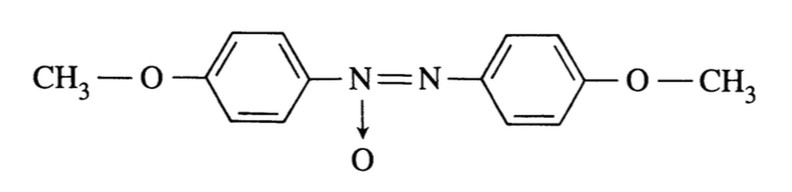
\includegraphics[width=\textwidth]{slike/nematic_molecule.png}
	\end{subfigure}
	\caption{\emph{Tipičen primer molekule, ki sestavlja snov z nematsko tekočekristalno fazo. Molekula ima podolgovato obliko z daljšo osjo dolgo $\approx 20$Å ter krajšo dolgo $\approx 5$Å.}}
	\label{fig:nematicmolecule}
\end{figure}

Tudi \emph{dvolomnost} nematikov je posledica lastnosti molekul iz katerih so sestavljeni. Odziv molekul na električno polje je večji za polja vzporedna osi kot za pravokotna, oziroma $\varepsilon_{||}^{mol} > \varepsilon_{\perp}^{mol}$. Takšna razlika je posledica delokaliziranosti elektronov v aromatskih obročih, ki jim omogoča več svobode gibanja kot elektronom vezanim na atome in zaradi vezi med njima, je prehajanje elektronov med njima zelo enostavno. Slednje je vzrok za močno anizotropijo v odzivu na električna polja, saj je polarizabilnost molekul v tej smeri višja kot v pravokotnih smereh. Tako je tudi za časovno odvisna polja frekvenc okoli vidnega dela spektra, torej za dielektričnost in posledično povzroči razliko med lomnima količnikoma običajno in neobičajno polarizirane svetlobe.\\

Razlike med izotropno in nematsko fazo najdemo v makroskopskih lastnostih takšnih snovi kot je na primer tenzor magnetne susceptibilnosti $\chi_{ij}$ ali pa tenzor dielektrične permitivnosti $\varepsilon_{ij}$. Slednji ima v enoosnem nematiku dve različni lastni vrednosti, ki jih bomo določili kasneje medtem ko so v izotropni fazi molekule orientacijsko neurejene, direktor ni definiran, zato je tudi $\varepsilon$ tam izotropen tenzor z eno samo lastno vrednostjo. Nas bo zanimalo predvsem, kako lahko konstruiramo tenzor, s katerim lahko opišemo stopnjo urejenosti v nematiku in ga kasneje povežemo s tenzorjem dielektričnosti (ali kako drugo makroskopsko količino). Za ta namen konstruiramo \emph{tenzor ureditvenega parametra} $Q_{ij}$, ki ga z $S$ in $\mathbf{n} = (n_x, n_y, n_z)$ zapišemo kot

\begin{equation}
Q_{ij} = \frac{S}{2}(3n_in_j-\delta_{ij}) + \frac{P}{2}\left (e_i ^{(1)}e_j^{(1)} - e_i^{(2)}e_j^{(2)} \right ).
\label{orderparametertensor}
\end{equation}

Tenzor vsebuje tudi možen prispevek \emph{biaksialnosti} $P$, ko molekule niso osno simetrične (imajo npr. ploščasto strukturo) ali pa zunanja vplivi, na primer električno polje ali robni pogoji na površini, porušijo osno simetrijo fluktuacij v nematiku. V tem primeru je $\mathbf{e}^{(1)} \perp \mathbf{n}$ \emph{sekundarni direktor} še ena smer v kateri pojavi urejanje molekul ter $\mathbf{e}^{(2)} = \mathbf{n} \times \mathbf{e}^{(1)}$. Biaksialnost $P$ leži v intervalu $[-3/2,3/2]$: $P=0$ pomeni zopet enoosni nematik, $|P|=3/2$ pa zgolj urejanje vzdolž sekundarnega direktorja. Tenzor $Q_{ij}$ je realen, simetričen ter je brez sledi -- $Q_{ii} = 0$\footnote{Pri zapisu sledi tenzorja $\tr A = A_{ii}$ uporabimo Einsteinovo sumacijsko konvencijo pri kateri je privzeto seštevanje po ponovljenem indeksu.}. Ima v splošnem 6 neodvisnih komponent vedno pa je moč najti osi koordinatnega sistema, oziroma lastne vektorje, v katerem je diagonalen in na njegovi diagonali ležijo lastne vrednosti

\begin{equation}
Q_{ij} = \begin{pmatrix} S & 0 & 0 \\
				0 & -\frac{1}{2}(S+P) & 0 \\
				0 & 0 & -\frac{1}{2}(S-P)	
	   \end{pmatrix}.
\label{uniaxialQ}
\end{equation}
Lastni vektorji pripadajoči lastnim vrednostim so direktor $\mathbf{n}$, sekundarni direktor $\mathbf{e}^{(1)}$ ter $\mathbf{e}^{(2)}$.

\subsection{Prosta energija nematikov}

Ravnovesna stanja fizikalnih sistemov so stanja v katerih je prosta energija najnižja. Gostota proste energije nematikov $f$ je v splošnem sestavljena iz različnih prispevkov

\begin{equation}
f = f_{NI} + f_{E} + f_S + ...,
\label{lcfe}
\end{equation}

kjer $f_{NI}$ opisuje prispevke k energiji zaradi orientacijske urejenosti v tekočem kristalu, $f_E$ prispevke zaradi deformacij direktorja, kot je na primer zvijanje ali upogibanje direktorja, $f_S$ pa morebitne prispevke zaradi robnih pogojev na stiku med nematikom in površino, kjer je smer direktorja vsiljena. \\

Običajni pristop k opisu faznega prehoda med neurejeno izotropno in delno urejeno nematsko fazo je zapis dela proste energije, ki se nanaša na fazni prehod $f_{NI}$, s pomočjo zgoraj definiranega tenzorja ureditvenega parametra $Q_{ij}$. V Landauovi teoriji faznih prehodov prosto energijo sistema zapišemo kot razvoj po potencah \emph{skalarnega} ureditvenega parametra. V primeru nematikov imamo opravka s \emph{tenzorjem} ureditvenega parametra zato iz njega tvorimo skalarne invariante t.j. količine, ki so v vseh koordinatnih sistemih v katerih lahko tenzor zapišemo enake. Osnovne invariante tenzorja $Q_{ij}$ so matrične sledi njegovih potenc do tretjega reda

\begin{equation}
Q_{ii}, \quad Q_{ij}Q_{ij}, \quad Q_{ij}Q_{jk}Q_{ki}.
\label{Qtraces}
\end{equation}

Da se pokazati, da je sled poljubne potence $3\times 3$ tenzorja $Q_{ij}$ moč zapisati zgolj kot linearno kombinacijo sledi (\ref{Qtraces}). Vemo, da je sam $Q_{ij}$ brezsleden, zato nam ostaneta zgolj drugi in tretji red\cite{gramsbergen}. Gostoto proste energije $f_{NI}$ lahko tedaj zapišemo kot potenčni razvoj do četrtega reda
\begin{equation}
f_{NI} = \frac{1}{2} A(T) Q_{ij}Q_{ij} + \frac{1}{3} B Q_{ij}Q_{jk}Q_{ki} + \frac{1}{4}(Q_{ij}Q_{ij})^2.
\label{landaufe}
\end{equation}
Koeficient $A(T) = a(T-T_{NI}^*)$ je snovni parameter, ki je temperaturno odvisen in vodi do faznega prehoda, $B < 0$ in $C > 0$ pa sta snovni konstanti. $T_{NI}^*$ je podhladitvena (\emph{supercooling}) temperatura, ki je blizu temperature faznega prehoda $T_{NI}$. Konstante so materialni parametri tipičnih vrednosti $a\sim 10^5J/(m^3K)$, $B\sim 10^6 J/(m^3)$ in $C\sim10^6J/m^3$\cite{ravnik}. Prosta energija (\ref{landaufe}) vsebuje tudi lihi prispevek v tretjem redu, kar pomeni da je opisani fazni prehod \emph{prvega reda} za katere je značilno, da pride pri temperaturi prehoda do nezveznega skoka v ureditvenem parametru. Vrednost $f_{NI}$ najbolj določa prvi člen: če je $A$ pozitiven je minimalna energija pri $Q=0$, kar opisuje izotropno fazo. V nasprotnem primeru, ko je $A$ negativen je $Q$, ki minimizira prosto energijo končen in določa nematsko fazo. Če v primeru enoosnega nematika ($P = 0$) vstavimo $Q$ v diagonalizirani obliki (\ref{uniaxialQ}) v enačbo (\ref{landaufe}) dobimo

\begin{equation}
f_{NI} = \frac{3}{4}A(T-T_{NI}^*)S^2 + \frac{1}{4}BS^3 + \frac{9}{16}CS^4.
\end{equation}

V tem izrazu lažje interpertiramo pomen posameznih prispevkov: prvi člen vodi do faznega prehoda, drugi vsebuje dejstvo da $S$ in $-S$ stanji nista ekvivalentni zadnji, pozitivni, člen pa zagotavlja, da je gostota proste energija omejena od spodaj. Vrednost $S$ v ravnovesju pri neki temperaturi $T$ najdemo tako, da minimiziramo ustrezno prosto energijo $F=\int f \dd V$ oziroma prek pogoja $\partial f_{NI}/\partial S = 0$. Dobimo ravnovesno vrednost $S_{rav} (T)$
\[   
S_{rav}(T) = 
     \begin{cases}
       0 &\quad T>T_{NI}\\
       \frac{1}{2} \left [-\frac{B}{3C} + \sqrt{\left (\frac{B}{3C} \right)^2 - \frac{8a(T-T_{NI}^*)}{3C}}  \right ] &\quad T<T_{NI} \\
       \label{Stransition}
     \end{cases}
\]

Slika \ref{fig:landau_F} prikazuje prosto energijo kot funkcijo stopnje urejenosti $S$ pri treh različnih temperaturah $T^{\dag}$, ki ustreza izotropni fazi, $T_{NI}$, ki je temperatura faznega prehoda ter $T^*$, ki ustreza nematski fazi. Na Sliki \ref{fig:landau_S} pa je prikazana še odvisnost $S$ od reducirane temperature $\tau$, ki doseže največjo možno vrednost ($\tau = 1$) pri $T_{NI}$: tam $S$ \emph{nezvezno} pade na 0\cite{gramsbergen}. Nezvezno razliko $S_0$ lahko izračunamo iz izraza (\ref{Stransition}) z izvrednotenjem pri $T= T_{NI}$.

\begin{figure}[h!]
	\centering
	\begin{subfigure}[b]{0.45\textwidth}
	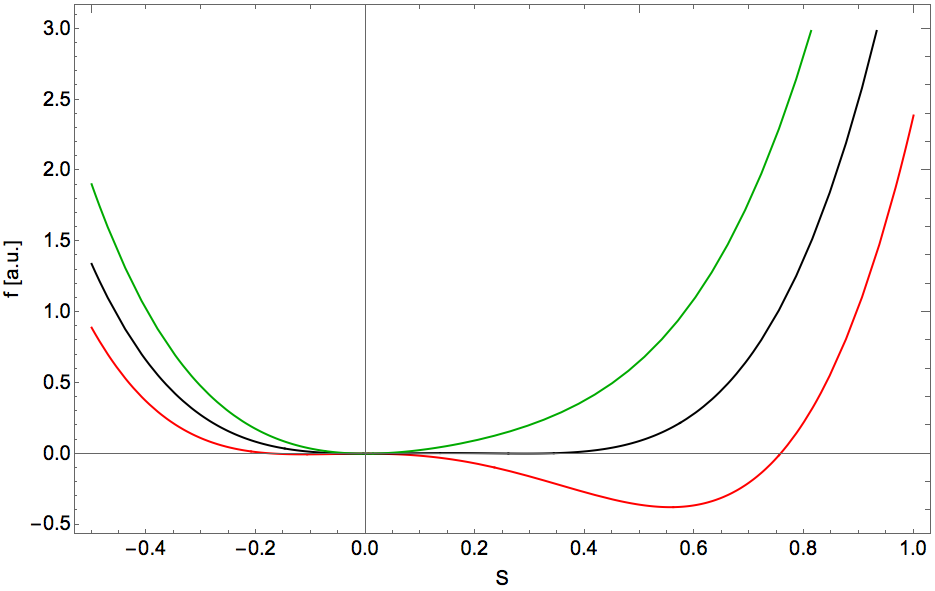
\includegraphics[width=\textwidth]{slike/landau_PT_F_my.png}
	\phantomcaption
	\label{fig:landau_F}
	\end{subfigure}
	\begin{subfigure}[b]{0.45\textwidth}
	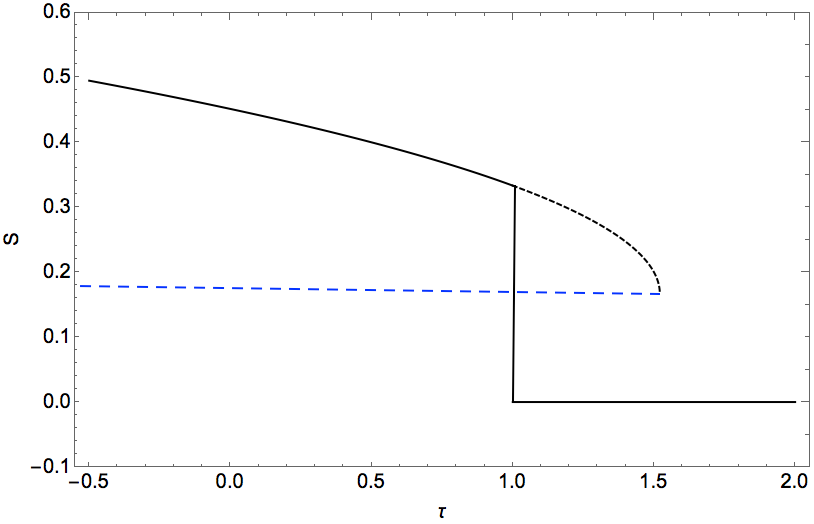
\includegraphics[width=\textwidth]{slike/landau_PT_S_my.png}
	\phantomcaption
	\label{fig:landau_S}
	\end{subfigure}
	\caption{\emph{\textbf{a.)} Prosta energija $f_{NI}$ v odvisnosti od ureditvenega parametra $S$ za tri različne temperature v okolici temperature faznega prehoda $T_{NI}$. \textbf{b.)} Nematski red $S$ v odvisnoti od reducirane temperature $\tau$ v nematski fazi. Ko $\tau = 1$ pri temperaturi $T_{NI}$ ima $S$ nezvezen skok. Vir slike:\cite{gramsbergen}}}
\end{figure} 

Naslednji pomembni prispevek k prosti energiji $f$ v enačbi (\ref{lcfe}) je prispevek zaradi prostorkega spreminjanja direktorja v nematiku $f_{E}$ -- deformacij. Takšne variacije $\mathbf{n}$ se dogajajo na razdaljah, ki so veliko večje ($\sim \mu$m) od velikosti posameznih molekul ($\sim $nm), zato je upravičen fenomenološki pristop z uporabo kontinuumske teorije, podobno kot opisujemo deformacije v trdni snovi. V Frank-Oseenovi teoriji proste energije so osnovne tri deformacije značilne za nematike  pahljačasta deformacija (\emph{splay}), zvijanje (\emph{twist}) ter upogibanje (\emph{bend}). Prispevek k prosti energiji je nato kar vsota posameznih deformacijskih energij s pripisanimi elastičnimi konstantami $k_i$
\begin{equation}
f_{NE} = f_0 + k_1 (\nabla \cdot \mathbf{n})^2 + k_2(\mathbf{n} \cdot \nabla \times \mathbf{n} - q_0)^2 + k_3 (\mathbf{n} \times \nabla \times \mathbf{n})^2.
\label{frankfe}
\end{equation}

V tej enačbi je $q_0 = 2\pi /p_0$ in $p_0$ razdalja v kateri se direktor v kiralnem tekočem kristalu, kot je na primer holesterična faza, (glej \ref{fig:liquidcrystaltypes}c) zavrti za polni kot $2\pi$ in $q_0 = 0$ v običajnem nematiku. Elastične konstante lahko določimo z eksperimentom. Opisane tri deformacije so prikazane na Sliki \ref{fig:lcdeformations}. 
\begin{figure}[h!]
	\centering
	\begin{subfigure}[b]{0.7\textwidth}
	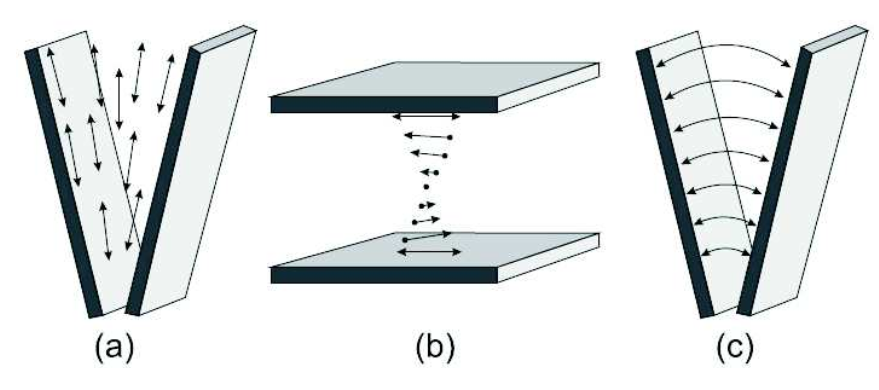
\includegraphics[width=\textwidth]{slike/lc_deformations.png}
	\end{subfigure}
	\caption{\emph{Tri osnovne deformacije v nematiku: pahljačasta deformacija, zvijanje in upogibanje direktorja.}}
	\label{fig:lcdeformations}
\end{figure}

Prispevek k prosti energiji zaradi deformacij je v tem kontekstu bolje zapisati s tenzorjem ureditvenega parametra $Q_{ij}$, ki je posredno povezan z $\mathbf{n}$ -- glej (\ref{orderparametertensor}). Ker gre pri deformacijah direktorja za krajevne spremembe v $Q_{ij}$ iščemo krajevne odvode količine, ki bo invariantna na spremembo koordinatnega sistema -- tudi v tem primeru je to sled potenc $Q_{ij}$. 

\begin{equation}
f_E = \frac{1}{2} L_1 \frac{\partial Q_{ij}}{\partial x_k}\frac{\partial Q_{ij}}{\partial x_k} + \frac{1}{2} L_2  \frac{\partial Q_{ij}}{\partial x_j}\frac{\partial Q_{ik}}{\partial x_k} + \frac{1}{2}L_3Q_{ij}  \frac{\partial Q_{kl}}{\partial x_i}\frac{\partial Q_{kl}}{\partial x_j}
\label{Qfe}
\end{equation}

Konstante $L_i$ je s primerjavo z izrazom (\ref{frankfe}) moč izraziti s konstantami $k_i$, ki so direktno povezane s posameznim tipom deformacije in so zato na nek način bolj naravne. Še bolj ključno pa je, da so $k_i$ pogosto primerljive velikosti in v tem primeru v izrazu (\ref{Qfe}) znatno prispeva zgolj prvi člen z $L_1$, ki opisuje vse tri osnovne deformacije. Gostoto elastične energije v približku ene konstante za nematik tako zapišemo kot
\begin{equation}
f_E = \frac{1}{2} L \frac{\partial Q_{ij}}{\partial x_k}\frac{\partial Q_{ij}}{\partial x_k}.
\label{Qfeone}
\end{equation}
Ker $Q_{ij}$ vsebuje tako $\mathbf{n}$ kot $S$ takšen elastičen člen opisuje tako deformacije direktorja kot tudi stopnje reda, kar je ključno za opis defektov, kjer pade $S$ na nič in direktor postane nedefiniran. 

Omeniti moramo tudi, kako se spremeni opis v kiralni fazi, saj bo to v nadaljevanju pomembno. Zaradi zvijanja direktorja dodamo enačbi (\ref{Qfeone}) še en člen povezan z zgoraj omenjenim $q_0$. Celotno gostoto energije kiralne faze nato napišemo kot
\begin{equation}
f^{chiral}_{E} =  \frac{1}{2} L \frac{\partial Q_{ij}}{\partial x_k}\frac{\partial Q_{ij}}{\partial x_k} + 2q_0L\epsilon_{ikl}Q_{ij}\frac{\partial Q_{ij}}{\partial x_k},
\label{chiralfe}
\end{equation}
kjer je $\epsilon_{ikl}$ popolnoma antisimetričen tenzor določen s permutacijo indeksov. Ta zaradi simetrije nastopa zgolj v kiralnih nematikih, saj ti, kot pove že njihovo ime, niso invariantni na zrcaljenje prostora.\\

Kadar imamo nematik v stiku z neko površino se lahko zgodi t.i. \emph{površinsko sidranje}. To je pojav, ko ima del nematika, ki je v stiku s površino, zaradi njenih strukturnih ali kemijskih lastnosti, tam vsiljeno smer direktorja zato je energijsko bolj ugodno, če direktorsko polje tam drugačno kot daleč proč od površine. To se zgodi zaradi površinskega prispevka $f_S$ k gostoti proste energije, ki ga pogosto opišemo s t.i. Ramini-Papoular modelom. V tem modelu opisujemo deformacije, različne od želene površinske deformacije opisane s tenzorjem $Q_0$ s prispevkom k prosti energiji
\begin{equation}
f_S = \frac{W}{2}(Q-Q_0)^2,
\end{equation}
kjer je $W$ konstanta, ki opisuje kako močen je ta površinski efekt. \\

Zadnji in morda najpomembnejši prispevek k prosti energiji, ki ga bomo omenili je prispevek zaradi interakcije z električnim oziroma magnetnim poljem v katerega postavimo nematik. Molekule v nematiku navadno nimajo znatnega električnega dipolnega momenta. Energijo nematika v zunanjem električnem polju $\mathbf{E}$ zato zapišemo v komponentnem zapisu kot
\begin{equation}
f_E = -\frac{1}{2}\varepsilon_{ij} E_iE_j.
\label{electricfieldfreeE}
\end{equation}
V nematikih velja, da je zveza med tenzorjem dielektrične permitivnosti $\varepsilon_{ij}$ ter tenzorjem ureditvenega parametra $Q_{ij}$ enaka
\begin{equation}
\varepsilon_{ij} = \bar \varepsilon + \frac{2}{3} \varepsilon_{a}^{mol} Q_{ij},
\label{permitivityorder}
\end{equation}
kjer je $\bar \varepsilon$ izotropni del $\varepsilon_{a}^{mol}$ pa anizotropni del \emph{molekulske} električne permitivnosti.\footnote{V makroskopskem nematiku velja, da je $\varepsilon_a =S \varepsilon_{a}^{mol}$, vendar je $S$ že vključen v $Q_{ij}$.} Če izraz (\ref{permitivityorder}) vstavimo v (\ref{electricfieldfreeE}) dobimo
\begin{equation}
f_E = -\frac{1}{2}\bar \varepsilon E^2 - \frac{1}{3} \varepsilon_a^{mol} Q_{ij} E_i E_j.
\end{equation}
Električno polje poskuša molekule poravnati s samim seboj ali pa pravokotno nanj odvisno od vrednosti anizotropije nematika $\varepsilon_a^{mol}$. Če $\varepsilon_a^{mol}<0$ se bodo molekule skušale poravnati pravokotno na smer polja in s tem material postane dvoosen\cite{gramsbergen}. Tipično molekula v nematiku potrebuje nekaj milisekund, da se odzove na zunanje električno polje. To pomeni, da nematik ne mora slediti na primer frekvenčno odvisnemu polju vidne svetlobe pač pa se tam poravna z efektivnim električnim poljem, ki ga opišemo z intenzitetnim tenzorjem svetlobe
\begin{equation}
I_{ij} = \frac{1}{2} \langle E_i E_j \rangle.
\end{equation}
Energijo dielektrične interakcije nematika s svetlobo nato zapišemo
\begin{equation}
f_D = -\frac{2}{3}\varepsilon_{a}^{mol} I_{ij}Q_{ij}.
\end{equation}
Takšen člen v prosti energiji omogoča opisovanje in modeliranje primerov, ko z visoko intenzitetnimi žarki preurejamo direktor v nematiku in ustvarimo defekte\cite{cancula,cancula2}.

%-------defekti---------%
\subsubsection{Defekti}

S pojmom defekti označujemo območja v nematikih, kjer je direktorsko polje $\mathbf{n}(\mathbf{r})$ nezvezno. Direktorja tam ne moremo definirati, skalarni parameter reda $S$ pa (zvezno) pade na nič, kot v izotropnih materialih. Defekti se v nematikih pojavijo zaradi različnih razlogov na primer površin ali pa zunanjih polj, ki vsiljujejo smer direktorja. V 3D strukturah se defekti lahko pojavijo v obliki posameznih točk ali pa defektnih linij (\emph{disclinations}). Ker se v okolici takšnih struktur tako $S$ kot $\mathbf{n}$ spreminjata hitreje, kot v preostalem nematiku, takšna območja stanejo veliko proste energije\cite{lavrenovitch}. \\

Matematična lastnost, ki jo pripišemo defektom je t.i. \emph{ovojno število} (\emph{winding number}) $s$, ki pove, koliko obratov naredi direktor na zanki okoli defekta. Ker sta obe usmeritvi direktorja $\mathbf{n} = -\mathbf{n}$  enakovredni so v nematikih možna le celoštevilska in polcela ovojna števila\cite{lavrenovitch}. Za različne vrste defektov je tipično tudi obnašanje optične osi okoli njih, v središču defekta, kjer je direktor nedefiniran, pa material postane lokalno izotropen.

\subsection{Širjenje svetlobe v nematikih} 

Tenzor dielektričnosti $\varepsilon_{ij}$ je v nematikih direktno povezan z tenzorjem ureditvenega parametra $Q_{ij}$ prek enačbe (\ref{permitivityorder}). Drugi člen v tej enačbi predstavlja anizotropni del tenzorja, prisoten zgolj v nematski fazi, ko $Q_{ij} \neq 0$. Ker je anizotropni del tenzorja $\varepsilon_{ij}$ sorazmeren $Q_{ij}$ si tenzorja delita enake lastne osi. V primeru enoosnega nematika to pomeni, da sta zanj značilni dve lastni vrednosti $\varepsilon$ in pripadajoče lastne osi: $\varepsilon_{||}$, ki jo občuti svetloba polarizirana vzdolž direktorja $\mathbf{n}$ ter $\varepsilon_{\perp}$ za svetlobo polarizirano v pravokotni ravnini, ki jo določa direktor. 
Ker velja, da je lomni količnik $n_i = \sqrt{\varepsilon_{ii}}$ sledi, da ločimo v nematikih tudi dva različna lomna količnika in sicer \emph{rednega} $n_o = \sqrt{\varepsilon_{\perp}}$ ter \emph{izrednega} $n_e = \sqrt{\varepsilon_{||}}$. Večina nematikov je pozitivno dvolomna, torej razlika med rednim in izrednim lomnim količnikom $\Delta n = n_o - n_e > 0$ obstajajo pa tudi primeri negaitvne dvolomnosti $\Delta n < 0$ in ti bodo za nas bolj zanimivi.\\

Z defekti v nematikih lahko vplivamo na polarizacijski in fazni profil svetlobnega snopa. Defektna linija z ovojnim številom $s$ lahko linearno polariziraci snop svetlobe spremeni v snop svetlobe z vektorsko polarizacijo, na kateri je odtisnjen defekt z močjo $2s$, kar lahko pokažemo z Jonesovim formalizmom\cite{cardano} še več pa nam pove modeliranje z FDTD metodo. Z njo namreč lahko napovemo tudi kako pride do intenzitetne ničle v sredini snopa pri taki pretvorbi\cite{cancula2}. Možen je tudi obratni proces, ko močni žarki preurejajo nematik\cite{cancula}. Nadalje, lahko svetlobni nosi tako spinsko vrtilno količino, ki se kaže kot krožna polarizacija svetlobe, kot tudi orbitalno vrtilno količino (OAM), če ima fazno nezveznost v središču. Nekateri nematski defekti omogočajo pretvorbo enega tipa vrtilne količine v drugo in s tem pripraven način za tvorbo žarkov z vrtinčno fazo\cite{marrucci}. 

\subsection{Holesteriki in modre faze}

Nematike, ki jih sestavljajo \emph{kiralne} molekule, torej takšne ki niso invariantne na obrat prostora, imenujemo \emph{holesteriki} oziroma kiralni nematiki. V nekaterih kiralnih nematikih na prehodu v izotropno fazo opazimo  t. i. \emph{helično fazo} (\emph{helical phase}), ki jo, nekoliko nehvaležno, prav tako pogosto imenujemo holesterična faza. Ta faza je prikazana na Sliki \ref{fig:liquidcrystaltypes}c. Zanjo je značilno nehomogeno direktorsko polje $\mathbf{n}(\mathbf{r})$: direktor je povsod pravokoten na os $\mathbf{\hat{a}}$ in homogen v vseh nanjo pravokotnih ravninah, a ko se premikamo vzdolž osi $\mathbf{\hat{a}}$, se direktor zvija okrog nje in se tipično zavrti za polni kot v nekaj desetinkah mikrometra. Takšno zvijanje direktorja lahko matematično opišemo, če poravnavmo os $\mathbf{\hat{a}}$ s koordinatno osjo $z$, saj je potem
\begin{equation}
\mathbf{n} (\mathbf{r}) = \mathbf{\hat{e}}_x \cos (q_0z) + \mathbf{\hat{e}}_y \sin(q_0z),
\end{equation}
kjer je $q_0=2\pi/p_0$ vijačnost, že omenjena količina, ki opisuje kako hitro se vzdolž $z$ direktor zvija -- $q_0$ je mera za \emph{kiralnost} nematika\cite{wright}.

Vendar pa opisana faza ni edina, ki jo opazimo v kiralnih nematikih. V kiralnih nematikih z visoko kiralnostjo $q_0$ se v sorazmerno ozkem temperaturnem območju pojavi t.i. modra faza -- BP (\emph{blue phase}). Kljub temu, da so modre faze sorazmerno neznačilne za tekoče kristale so v resnici eno izmed prvih odkritij na tem področju, saj jih je že leta 1888 odkril Reinitzer, ki je ohlajal holesterol benzoat. Pri neki temperaturi je opazil, da je substanca odsevala modro barvo, a je pojav hitro izginil. Kasneje so po tem pojavu fazo tudi poimenovali. \\

Da modre faze odbijajo različne frekvence svetlobe je posledica njihove periodične strukture, na kateri pride do Braggovega sipanja. Gre namreč za urejeno mrežo \emph{linijskih defektov}, ki nastanejo kot posledica lokalnega urejanja kiralnih molekul v t.i. \emph{dvojno-zvite cilindre} -- DTC (\emph{double-twist cylinder}). To so cilindrične strukture v katerih se zasuk direktorja glede na os cilindra linearno povečuje z oddaljenostjo od osi. Če kot med osjo cilindra in direktorjem opišemo s kotom $\chi(r)$ razdaljo med njima pa označimo z $r$ velja
\begin{equation}
\chi(r) = \frac{\pi}{4} \frac{r}{R} = q_0 r,
\end{equation}
kjer smo s $q_0$ zopet označili vijačnost, ki sedaj opisuje zvijanje v radialni smeri.
Na osi cilindra z radijem $R$ je direktor poravnan z osjo, potem pa se v vseh azimutalnih smereh $\phi$ linearno z $r$ zavrti do kota $\pi/4$. Matematično lahko DTC strukturo opišemo z vektorskim poljem v cilindričnih koordinatah kot
\begin{equation}
\mathbf{n}(r, \varphi, z) = \mathbf{e}_z \cos (q_0r)  -   \mathbf{e}_\varphi \sin (q_0r).
\label{dtcdirector}
\end{equation}

Opisana struktura je prikazana na Slikah \ref{fig:dtc} ter \ref{fig:dtc_z}, kjer je prikazan pogled na en sloj DTC od zgoraj.\\

\begin{figure}[h!]
	\centering
	\begin{subfigure}[b]{0.4\textwidth}
	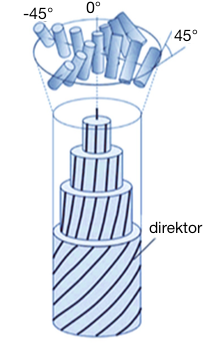
\includegraphics[width=\textwidth]{slike/double_twist_cylinder.png}
	\phantomcaption
	\label{fig:dtc}
	\end{subfigure}
	\begin{subfigure}[b]{0.5\textwidth}
	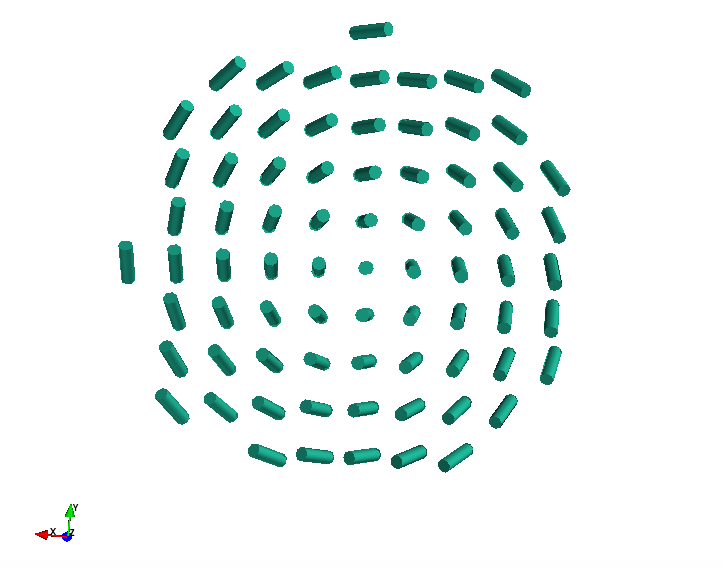
\includegraphics[width=\textwidth]{slike/dtc_z.png}
	\phantomcaption
	\label{fig:dtc_z}
	\end{subfigure}
	\caption{\emph{Dvojno-zviti cilinder ter en sloj iz ptičje perspektive.}}
\end{figure}

Fazni prehod v modre faze lahko matematično opišemo z običajnim Landauovim prispevkom k prosti energii (\ref{landaufe}) ter z opisanim elastičnim prispevkom v kiralnih nematikih (\ref{chiralfe}). Ta dva prispevka združeno vodita do modrih faz, ki za primerne vrednosti parametrov minimizirajo prosto energijo. Iz gornjih enačb lahko v limiti visoke kiralnosti $q_0\rightarrow \infty$ dobimo analitični tenzor ureditvenega parametra v modrih fazah\cite{wright}. Eksperimentalno je sicer kiralnost $q_0$ v modrih fazah nizka in sicer med vrednostima $0.01$ ter $0.5$\cite{wright}.\\

Takšne strukture so v nematikih energijsko stabilne le za kratke razdalje glede na velikost celotne strukture: tipične vrednosti $R$ v modrih fazah so $\sim 100$nm. V modrih fazah se DTC naložijo v višje urejene strukture, na mestih kjer se cilindri srečajo pa nastanejo defekti, kar je prikazano na Slikah \ref{fig:dtcdefect1} ter \ref{fig:dtcdefect2}. Prikazana dva različna možna defekta: tip defekta določa \emph{sučnost} t.j. smer v kateri se direktor vrti okoli osi na mestu srečanja. Tako dobimo defekta z različno močjo, v prvem primeru gre za $s=1/2$ v drugem pa za $s=1$.
\begin{figure}[h!]
	\centering
	\begin{subfigure}[b]{0.4\textwidth}
	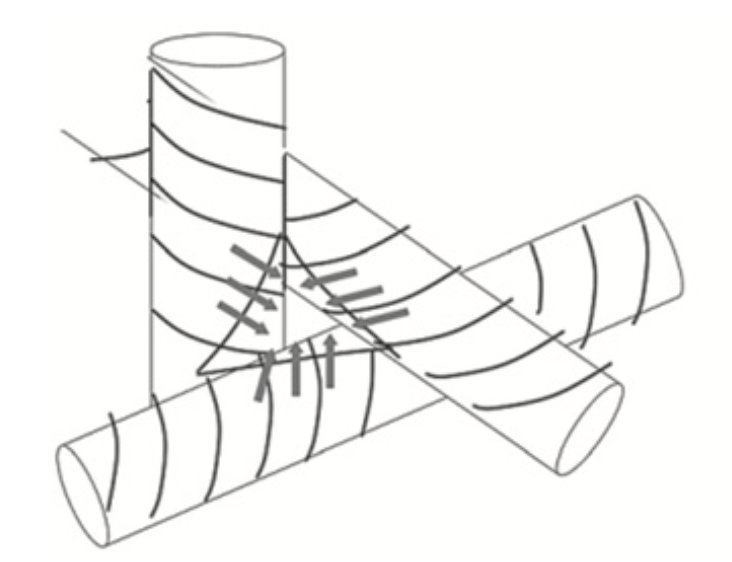
\includegraphics[width=\textwidth]{slike/dtc_defect_1.png}
	\phantomcaption
	\label{fig:dtcdefect1}
	\end{subfigure}
	\begin{subfigure}[b]{0.4\textwidth}
	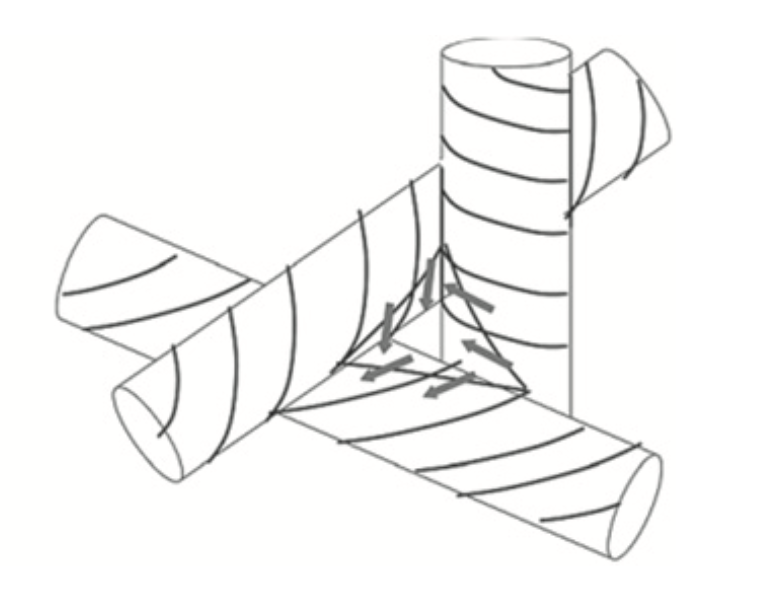
\includegraphics[width=\textwidth]{slike/dtc_defect_2.png}
	\phantomcaption
	\label{fig:dtcdefect2}
	\end{subfigure}
	\caption{\emph{Možna tipa defektov določena z lokalno smerjo vrtenja direktorja v udeleženih cilindrih. Na levi je prikazan defekt z nabojem $s = 1/2$ na desni pa z $s=1$. Vir slike:}}
\end{figure}
 
 Glede na strukturo naloženih cilindrov poznamo ločimo tri tipe modrih faz poimenovanih BP I, BP II ter BP III. BP III je amorfna faza kjer so cilindri neurejeni. V BP I in BP II tvorijo mesta, kjer se cilindri srečujejo  bodisi telesno centrirano (BCC) ali preprosto kubično (SC) mrežo, z velikostjo osnovne celice nekaj sto nanometrov. Takšne razdalje pa so razlog, da pride do konstruktivne interference valovanja za valovne dolžine v območju vidne svetlobe. Na Slikah \ref{fig:bp1} ter \ref{fig:bp2} sta prikazani strukturi BP I ter BP 2, kjer so z modro barvo prikazani dvojno-zviti cilindri, z rdečimi črtami pa so označeni linijski defekti, ki se prepletajo med njimi.\\
 
 \begin{figure}[h!]
	\centering
	\begin{subfigure}[b]{0.45\textwidth}
	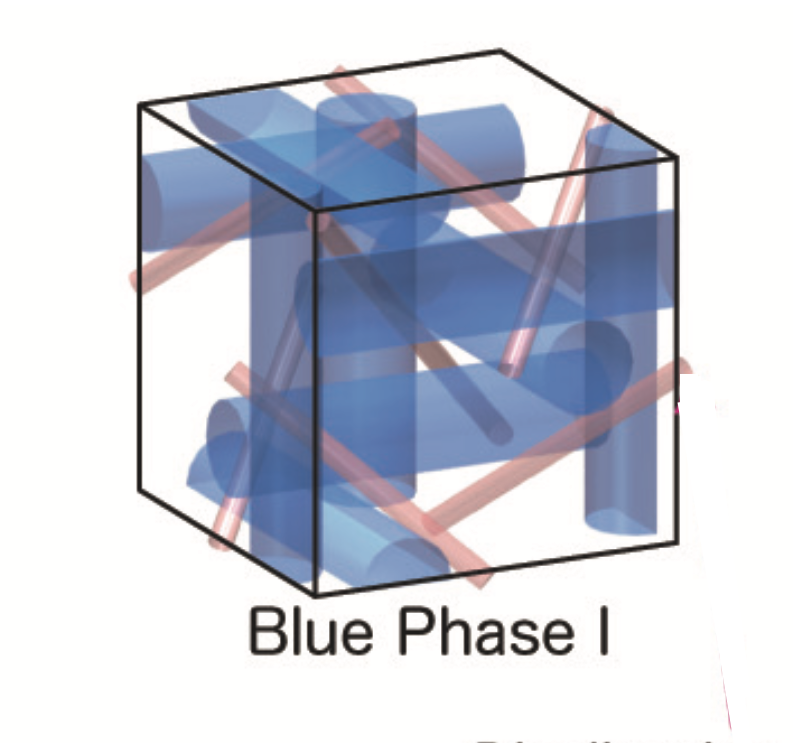
\includegraphics[width=\textwidth]{slike/bp_I.png}
	\phantomcaption
	\label{fig:bp1}
	\end{subfigure}
	\begin{subfigure}[b]{0.45\textwidth}
	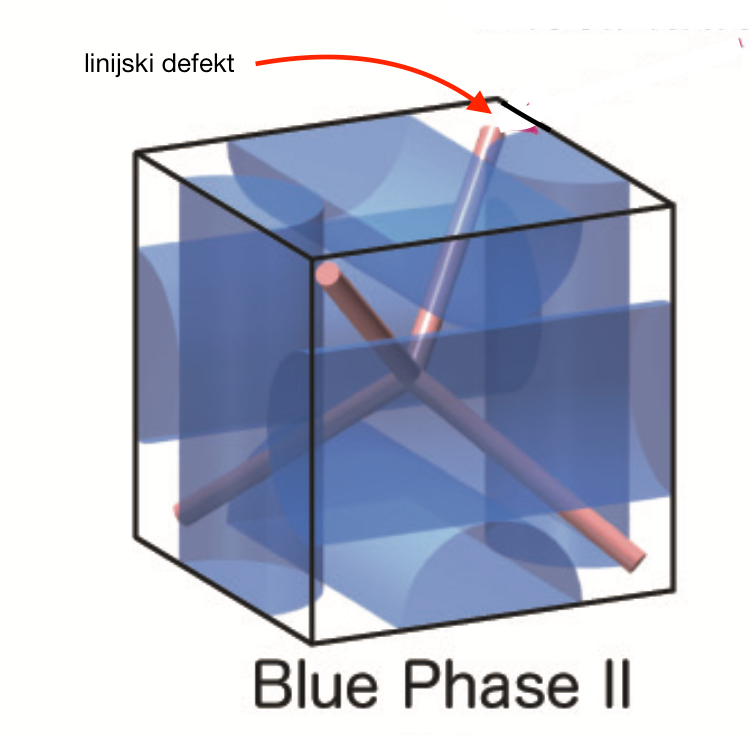
\includegraphics[width=\textwidth]{slike/bp_II.png}
	\phantomcaption
	\label{fig:bp2}
	\end{subfigure}
	\caption{\emph{Shematski prikaz osnovne celice tipov modrih faz BP I (FCC mreža) ter BP II (SC mreža). Z modro barvo so prikazani dvojno zviti cilindri z rdečo pa defektne linije. Vir slike: }}
\end{figure}

Ker mrežo tvorijo defekti takšna struktura ni zelo stabilna, kar je tudi razlog za običajno relativno ozko temperaturno območje (reda 1K), kjer take faze sploh obstajajo. To nekoliko otežuje njihovo potencialno uporabo, zato se v zadnjih letih veliko truda vlaga v razvoj modrih faz, ki so stabilne v širšem temperaturnem območju. Leta 2005 so odkrili prvi tekoči kristal, v katerem modri fazi BP I ter BP II obstajata v temperaturnem območju od $16^\circ$ do $50^\circ$ C\cite{coles}. Poleg odkrivanja novih materialov je možno modre faze tudi \emph{stabilizirati} z dodatkom polimerov ali koloidov\cite{kikuchi,ravnik2, ravnik3}. Ena izmed lastnosti modrih faz, ki jih dela zanimive, je hiter odzivni čas na zunanje električno polje, reda 10-100 mikrosekund, kar je nekajkrat hitreje od običajnih nematikov. To obeta razvoj novih tipov tekočekristalnih zaslonov od katerih si obetamo hitrejši čas osveževanja (\emph{refresh rate}) ter boljšo ločljivost\cite{kikuchi2}.




%%%----------------------RAČUNSKA METODA----------------%
\chapter{Računska metoda}

Obstaja več različnih numeričnih metod s katerimi lahko opisujemo elektromagnetno valovanje. Izbira metode je odvisna od več faktorjev: tipične dimenzije objektov v simulaciji, relevantnih časovnih dimenzij, frekvence oziroma valovne dolžine svetlobe, \emph{itn}. Pomembno je tudi, katere lastnosti svetlobe nas pri določenem problemu sploh zanimajo.

V fiziki tekočih kristalov nas pogosto zanima le polarizacija svetlobe in kako se ta spreminja vzdolž poti žarkov. Za opis takšnih problemov je najbolj preprosta metoda, \emph{metoda Jonesovih matrik}. Ta predpostavlja širjenje svetlobe vzdol ene smeri, osi $z$, konstantno frekvenco svetlobe, ter optični polji $\mathbf{E}$ in $\mathbf{H}$, ki sta vedno pravokotni na smer širjenja svetlobe. Polarizacijo svetlobe na mestu $z$ potem opišemo zgolj s tremi vrednostmi, $E_x(z)$, $E_y(z)$ ter faznim zamikom $\phi$ med njima kar simbolično zapišemo z vektorjem, nato pa pot svetlobe skozi različne optične elemente, ki spreminjajo polarizacijo oopišemo z matrikami velikosti $2\times2$\cite{jones}.  Jonesov formalizem odpove, ko gre za opis delno polarizirane ali nepolarizirane svetlobe. Takrat lahko posežemo po splošnejši \emph{Muellerjevi metodi} v kateri splošno stanje polarizacije svetlobe je moč opisati z 4-komponentnimi \emph{Stokesovimi vektorji}, optične elemente pa z $4 \times 4$ matrikami\cite{stallinga}. 
Če se pa vselej zanimamo zgolj za popolnoma polarizirano svetlobo je generalizacija Jonesove metode \emph{Berremanova metoda}, ki poleg komponent električnega polja uporablja tudi komponente magnetnega. S takšno metodo lahko računamo tudi tok svetlobe prek meje dveh medijev, na način, ki upošteva robne pogoje za električno in magnetno polje. Na nobeno izmed opisanih metod pa se ne moramo upreti, kadar nas poleg polarizacije zanima tudi, kakšen vpliv imajo na širjenje snopa uklon ali kateri drugi valovni pojavi.\\

Zelo pomembno področje, pri katerem se numerične metode veliko uporablja so optični vodniki. Za računanje lastnih načinov razširjanja svetlobe skozi optična vlakna ali druge podobne strukture, se pogosto uporablja metoda VBP (\emph{vector beam propagation method}). Predpostavka, na kateri metoda gradi, je da imamo eno samo smer razširjanja svetlobe, vzdolž katere se amplituda ne spreminja znatno na razdaljah primerljivih z valovno dolžino svetlobe (\emph{slowly varying amplitude}). Metoda uporablja diskretno prostorsko mrežo, ki jo na enem koncu napolnemo z vsemi šestimi komponentami elektromagnetnih polj ($\mathbf{E}$ in $\mathbf{H}$). Polja nato propagiramo po mreži z reševanjem \emph{valovne enačbe} na vsakem koraku. Metoda je pogosto uporabljena v kombinaciji z metodo končnih elementov (\emph{finite-elements method}), ki omogoča boljšo diskretizacijo prostora in modeliranje kompleksnejših regij v prostoru\cite{pedrola}.\\

Metoda končnih diferenc v časovni domeni oziroma FDTD (\emph{finite-difference time-domain method}) je gotovo najbolj splošna od predstavljenih metod in najbolj široko uporabljena metoda za reševanje Maxwellovih enačb. Je popolnoma eksplicitna in sorazmerno preprosto razumljiva. Ker za računanje na vsakem koraku uporablja vse komponente polj v vseh točkah diskretne mreže računalniki hitro trčijo ob pomanjkanje spomina vendar ji ta ista lastnost omogoča modeliranje elektromagnetnega valovanja v praktično vseh medijih, kot so disperzivni (frekvenčno odvisen lomni količnik), anizotropni, kiralni ali nelinearni\cite{gedney}.\\

Metoda FDTD ni več nova, njeni začetki namreč segajo že v leto 1969. Pa vendar njena raba iz leta v leto narašča, o čemer priča tudi vedno večje število podjetij (npr. Lumerical, Remcom, Optiwave,...) s svojo programsko opremo za modeliranje svetlobe s pomočjo te metode\cite{gedney}. Večina programov je naravnana precej ciljno, torej namenjena zgolj reševanju enačb v določenem primeru na primer računanju lastnih načinov v valovnem vodniku ali sipanju svetlobe. Tako ne omogočajo modeliranja toka svetlobe skozi nehomogene anizotropne materiale kot so lahko tekoči kristali.

%%%%%----------------------METODA KONČNIH DIFERENC V ČASOVNI DOMENI----------%%%

\section{Metoda končnih diferenc v časovni domeni}

Za popoln opis elektromagnetnega polja potrebujemo dve vektorski polji: električno polje $\mathbf{E}$ ter magnetno polje $\mathbf{H}$, ter njuma ustrezni gostoti polj $\mathbf{D}$ in $\mathbf{B}$. Polja so medsebojno povezana s konstituitivnimi relacijami (\ref{constituitive}). Pri metodi FDTD gre v preprostem primeru, ko v prostoru ni izvorov električnih in magnetnih polj ter absorpcije, za reševanje časovno in prostorsko diskretiziranih Maxwellovih enačb (\ref{maxwell}), ki vsebujejo rotor $\nabla \times$
\begin{equation}
\epsilon \frac{\partial \mathbf{E}}{\partial t} = \nabla \times \mathbf{H}, \quad \mu \frac{\partial \mathbf{H}}{\partial t} = - \nabla \times \mathbf{E}.
\label{maxwelldiscrete}
\end{equation}
Ti dve enačbi narekujeta \emph{časovni razvoj} obeh polj. Drugi dve Maxwellovi enačbi, oziroma Gaussova zakona za obe gostoti polj, sta nujna posledica (\ref{maxwelldiscrete}), a moramo pri diskretizaciji paziti, da izberemo mrežo na kateri bosta implicitno upoštevani. FDTD metoda je drugačna, saj namesto valovne enačbe (\ref{waveequationE}) za $\mathbf{E}$ ali $\mathbf{H}$ rešuje sklopljeni enačbi za obe polji. \\

Metoda FDTD temelji na diskretizaciji časovnih in prostorskih odvodov v obliki \emph{končnih diferenc} v simetrični obliki\cite{schneider}. Če zapišemo Taylorjev razvoj skalarne funkcije ene spremenljivke $f(x)$ okoli točk $x_0 \pm \delta/2$
\begin{align}
f \left (x_0 + \frac{\delta}{2} \right) = f(x_0) + \frac{\delta}{2} f'(x_0) + \frac{1}{2!} \left ( \frac{\delta}{2} \right )^2 f''(x_0) + \frac{1}{3!} \left ( \frac{\delta}{3} \right )^3 f'''(x_0) + ... \\
f\left (x_0 - \frac{\delta}{2} \right ) = f(x_0) - \frac{\delta}{2} f'(x_0) + \frac{1}{2!} \left ( \frac{\delta}{2} \right )^2 f''(x_0) - \frac{1}{3!} \left ( \frac{\delta}{3} \right )^3 f'''(x_0) + ...
\end{align}
Ko odštejemo eno enačbo od druge in vse skupaj delimo z $\delta$ dobimo
\begin{equation}
 \frac{f \left (x_0 + \frac{\delta}{2} \right) -  f\left (x_0 - \frac{\delta}{2} \right)}{\delta} = f'(x_0)  + \frac{1}{3!} \frac{\delta^2}{4} f'''(x_0) + ..., 
\end{equation}
oziroma končna diferenca na levi strani enačbe, je enaka prvemu odvodu funkcije v točki $x_0$, ki mu prištejemo še člene, ki so višjega reda v $\delta$. Če je $\delta$ dovolj majhen lahko v linearnem približku vse višje člene zanemarimo in prve odvode nadomestimo z
\begin{equation}
\left .\frac{\dd f}{\dd x}\right |_{x=x_0} \approx  \frac{f \left (x_0 + \frac{\delta}{2} \right) -  f\left (x_0 - \frac{\delta}{2} \right)}{\delta}
\label{finitedifference}
\end{equation}
Iz enacbe (\ref{finitedifference}) vidimo, da za izračun odvoda funkcije $f$ v točki $x_0$ ne potrebujemo vrednosti funkcije v tej točki, pač pa zgolj vrednosti na sosednjih točkah $x_0 + \delta/2$ ter $x_0 - \delta/2$. Ker smo zanemarili vse člene z drugo ali višjo potenco $\delta$, pravimo, da ima ta približek natančnost drugega reda, obstajajo pa tudi približki višjih redov, ki za izračun potrebujejo več točk. Približek drugega reda (\ref{finitedifference}) je uporabljen tudi v naši implementaciji metode FDTD\cite{cancula}.

%----------Yeejev algoritem-------------%
\subsection{Yeejev algoritem}

Osnova večine implementacij metode FDTD je Yeejeva diskretacijska mreža. Prostor razdelimo v kubično mrežo tako, da sta polji $\mathbf{E}$ in $\mathbf{H}$ na njej spravljeni na različnih mestih in ob različnih časih. To je najlaže razložiti na enodimenzionalnem primeru: imejmo enodimenzionalno elektromagnetno valovanje potujoče v smeri $x$ in polarizirano v $z$ smeri. Polji tedaj zapišemo $\mathbf{E} = (0,0, E_z(x))$ in $\mathbf{H} = (0, H_y(x), 0)$ enačbi (\ref{maxwelldiscrete}) pa
\begin{equation}
\varepsilon \frac{\partial E_z}{\partial t}  = \frac{\partial H_y}{\partial x}, \qquad \frac{\partial H_y}{\partial t} = \frac{\partial E_z}{\partial x}.
\label{1Dcurleqs}
 \end{equation}
 Enačbi sedaj diskretiziramo, tako da vpeljemo diskretna prostorski $m$ ter časovni indeks $q$ z ustreznima korakoma $\Delta_x$ ter $\Delta_t$. Polje $E_z(x,t)$ tako pišemo
\begin{equation}
E_z(x,t) = E_z (m \Delta_x, q\Delta_t) = E_z^q [m],
\end{equation}
analogno pa velja za $H_y(x,t) \rightarrow H_y^q[m]$. Ker sta enačbi (\ref{1Dcurleqs}) sklopljeni ju je možno hkrati diskretizirati zgolj z uporabo posebne mreže, kot je tista prikazana na Sliki \ref{fig:staggeredfields}. Na njej sta polji $E_z$ in $H_y$ shranjeni na mestih medsebojno zamaknjenih za pol koraka tako v času kot v prostoru. S črtkano črto je na sliki označena meja med preteklostjo in prihodnostjo torej med že izračunanimi polji ter tistimi, ki jih še moramo izračunati. Ideja algoritma je, da mejo korak za korakom premikamo v prihodnost. Takšna razporeditev nam omogoča, da zapišemo enačbi (\ref{1Dcurleqs}) v diskretni obliki okoli označene točke
\begin{equation}
 \frac{H_y^{q+1/2}[m + 1/2] - H_y^{q-1/2}[m]}{\Delta_t} = \frac{E_z^q [m+1] - E_z^q [m]}{\Delta_x}.
\end{equation}
Kot vidimo, so vse količine razen ene v tej enačbi že znane (pod črtkano črto), zato lahko neznano količino izrazimo
\begin{equation}
H_y^{q+1/2} [m +1/2] = H_y^{q-1/2}[m] + \frac{\Delta_t}{\Delta_x} \left ( E_z^q[m+1] - E_z^q[m] \right ).
\label{updateH}
\end{equation}
Temu pravimo \emph{posodobitvena enačba} za magnetno polje v 1D primeru. Po izračunu magnetnega polja ob $q+1/2$ uporabimo še analogno enačbo za električno polje ob času $q+1$ v kateri nastopa ravnokar izračunano magnetno polje
\begin{equation}
E_z^{q+1} [m] = E_z^q [m] +\frac{\Delta_t}{\varepsilon \Delta_x}  \left (H_y^{q+1/2} [m+1/2] - H_y^{q+1/2} [m-1/2] \right ).
\label{updateE}
\end{equation}
Iteracije med obema posodobitvenima enačbama ponavljamo do želenega časa $t_0$.\\

Če povzamemo, sta obe posodobitveni enačbi (\ref{updateH}) ter (\ref{updateE}), da je računano polje v prihodnosti odvisno od istega polja v prejšnji točki v času z dodatkom člena, ki vsebuje vrednosti drugega polja v sosednjih točkah. Po vsaki uporabi se črtkana črta na Sliki \ref{fig:staggeredfields} premakne za pol časovnega koraka navzgor.

\begin{figure}[h!]
	\centering
	\begin{subfigure}[b]{0.45\textwidth}
	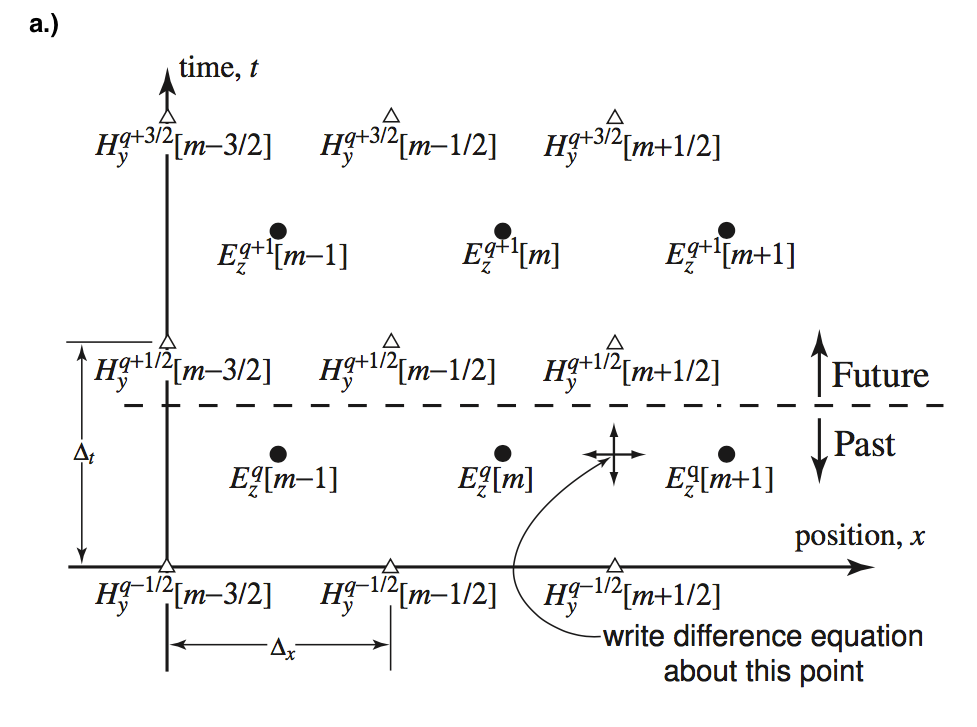
\includegraphics[width=\textwidth]{slike/staggered_fields.png}
	\phantomcaption
	\label{fig:staggeredfields}
	\end{subfigure}\quad
	\begin{subfigure}[b]{0.45\textwidth}
	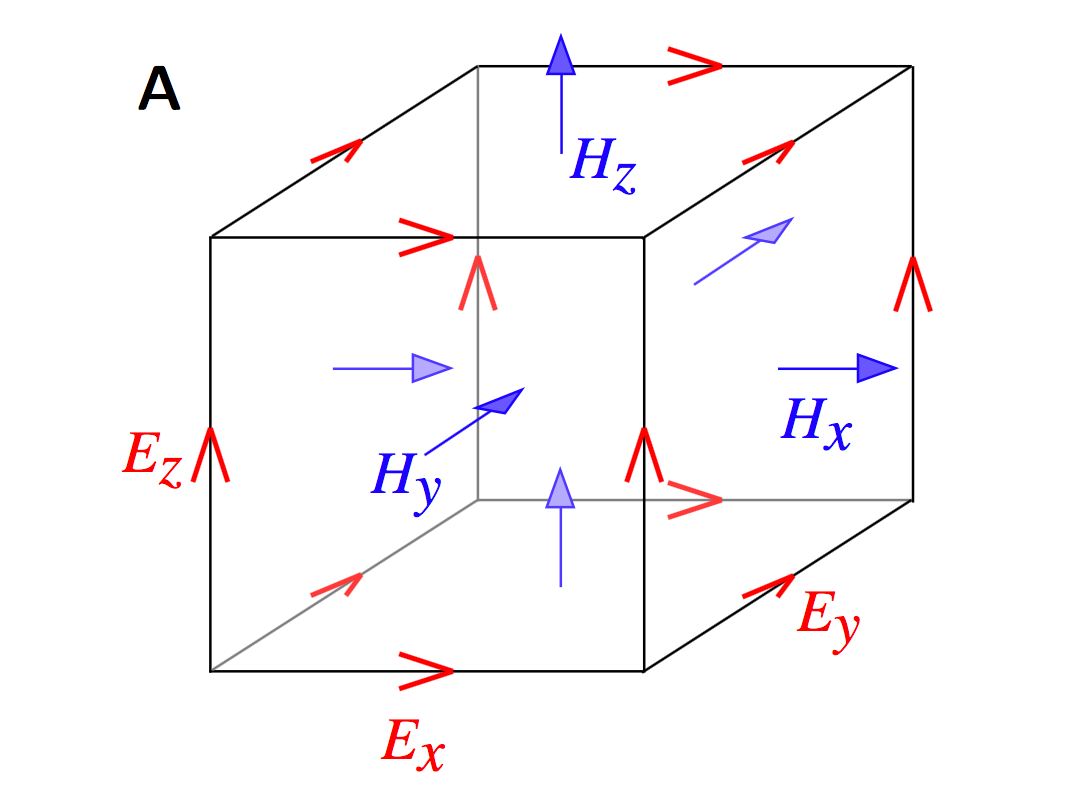
\includegraphics[width=\textwidth]{slike/yee_lattice_fields.png}
	\phantomcaption
	\label{fig:yeelattice}
	\end{subfigure}
	\caption{\emph{\textbf{a.)} Prikaz zamaknjenih polj v primeru enodimenzionalnega EM vala. \textbf{b.)} Yeejeva mreža za metodo FDTD v treh dimenzijah. Vir slik: \cite{lavrinenko, cancula}}}
\end{figure}

V treh dimenzijah razdelimo prostor na majhne kubične celice s stranico $\Delta_x$, vsaka z indeksom $(i,j,k)$. V vsaki izmed celic spravimo vseh šest komponent polja, na način prikazan na Sliki \ref{fig:yeelattice}. Na njej je prikazana \emph{ena sama} celica v Yeejevi mreži ob nekem časovnem trenutku $q$. Položaji v mreži, kjer so spravljene komponente magnetnega polja so ponovno za pol krajevnega in časovnega koraka zamaknjene glede na komponente električnega polja. Časovna zamaknjenost na tej sliki ni prikazana.\\

Z razporeditvijo komponent na ta način, dobimo diskretizacijo Maxwellovih enačb (\ref{maxwelldiscrete}), ki jih v homogenem anizotropnem materalu, kjer ima tenzor dielektričnosti zgolj diagonalne komponente, lahko razpišemo
\begin{align}
&\varepsilon_{xx} \frac{\partial E_x}{\partial t} = \frac{\partial H_z}{\partial y} - \frac{\partial H_y}{\partial z}, \qquad \mu \frac{\partial H_y}{\partial t} = \frac{\partial E_y}{\partial z} - \frac{\partial E_z}{\partial y} \\
&\varepsilon_{yy} \frac{\partial E_y}{\partial t} = \frac{\partial H_x}{\partial z} - \frac{\partial H_z}{\partial x}, \qquad \mu \frac{\partial H_y}{\partial t} = \frac{\partial E_z}{\partial x} - \frac{\partial E_x}{\partial z} \\
&\varepsilon_{zz} \frac{\partial E_z}{\partial t} = \frac{\partial H_y}{\partial x} - \frac{\partial H_x}{\partial y}, \qquad \mu \frac{\partial H_z}{\partial t} = \frac{\partial E_x}{\partial y} - \frac{\partial E_y}{\partial x}.
\label{3Dcurleqs} 
\end{align}

Za ponazoritev vzemimo odvoda $\partial E_y/\partial z$ ter $\partial E_z/\partial y$, ki sta ob uporabi končnih diferenc znana točno na mestu $H_y$, vendar samo ob časih $t_0-\Delta_t/2$ ter $t_0+\Delta_t/2$, kar pa je točno tisto kar potrebujemo za izračun $\partial H_y/\partial t$ ob času $t_0$. Enako velja za vseh šest zapisanih enačb. Uporaba take sheme torej omogoča, da ohranimo simetričnost diferenčne sheme, kar pomeni večjo stabilnost metode\cite{cancula}. Prav tako je moč pokazati, da sta v taki mreži implicitno upoštevani tudi preostali dve Maxwellovi enačbi\cite{taflove}.

\subsubsection{Anizotropni materiali}

Nehomogeno odvisnost dielektričnosti je mogoče vključiti v metodo prek diskretizacije $\varepsilon(\mathbf{r}) \rightarrow \varepsilon_{ijk}$. To je preprosto, kadar gre za izotropne materiale ali pa takšne anizotropne materiale, kjer se optična os ne spreminja in je tenzor diagonalen. Kot pa smo omenili pri poglavju o nematikih optično os anizotropije določa direktor, ki pa je pogosto močno krajevno odvisen -- spomnimo se na defekte. V takšnem primeru je tenzor $\varepsilon$ nediagonalen in krajevno odvisen zato diskretizacija Maxwellovih enačb na Yeejevi mreži ni več mogoča. Če namreč v enačbe za časovni razvoj električnega polja  (\ref{3Dcurleqs}) dodamo izvendiagonalne komponente $\varepsilon$ dobimo
\begin{align}
&\varepsilon_{xx} \frac{\partial E_x}{\partial t} + \varepsilon_{xy} \frac{\partial E_y}{\partial t} + \varepsilon_{xz} \frac{\partial E_z}{\partial t}= \frac{\partial H_z}{\partial y} - \frac{\partial H_y}{\partial z},\\
&\varepsilon_{yx} \frac{\partial E_x}{\partial t} + \varepsilon_{yy} \frac{\partial E_y}{\partial t} + \varepsilon_{yz} \frac{\partial E_z}{\partial t}= \frac{\partial H_x}{\partial z} - \frac{\partial H_y}{\partial x},\\ 
&\varepsilon_{zx} \frac{\partial E_x}{\partial t} + \varepsilon_{zy} \frac{\partial E_y}{\partial t} + \varepsilon_{zz} \frac{\partial E_z}{\partial t}= \frac{\partial H_y}{\partial x} - \frac{\partial H_x}{\partial y}.
\end{align}
Da dobimo celoten odvod polja $\partial \mathbf{E}/\partial t$ moramo za razliko od prej sedaj rešiti \emph{sistem} linearnih enačb. Poleg tega izgubimo prej opisane lastnosti Yeejeve mreže, saj za izračun katerekoli komponente $\mathbf{E}$ potrebujemo vse komponente $\mathbf{H}$. Zaradi tega mreža izgubi simetričnost diferenčne sheme in izgubi stabilnost\cite{werner}.\\

Če želimo ohraniti simetričnost ter smo pripravljeni žrtvovati nekaj več računskega časa, je moč metodo implementirati na mreži, ki to omogoča. Mesta, kjer so polja spravljena na naši mreži so prikazana na Sliki \ref{fig:ourlatticefields}, kjer je kjlučno opaziti, da so sedaj v vsaki točki mreže spravljene \emph{vse} tri komponente posameznega polja!

\begin{figure}[h!]
	\centering
	\begin{subfigure}[b]{0.45\textwidth}
	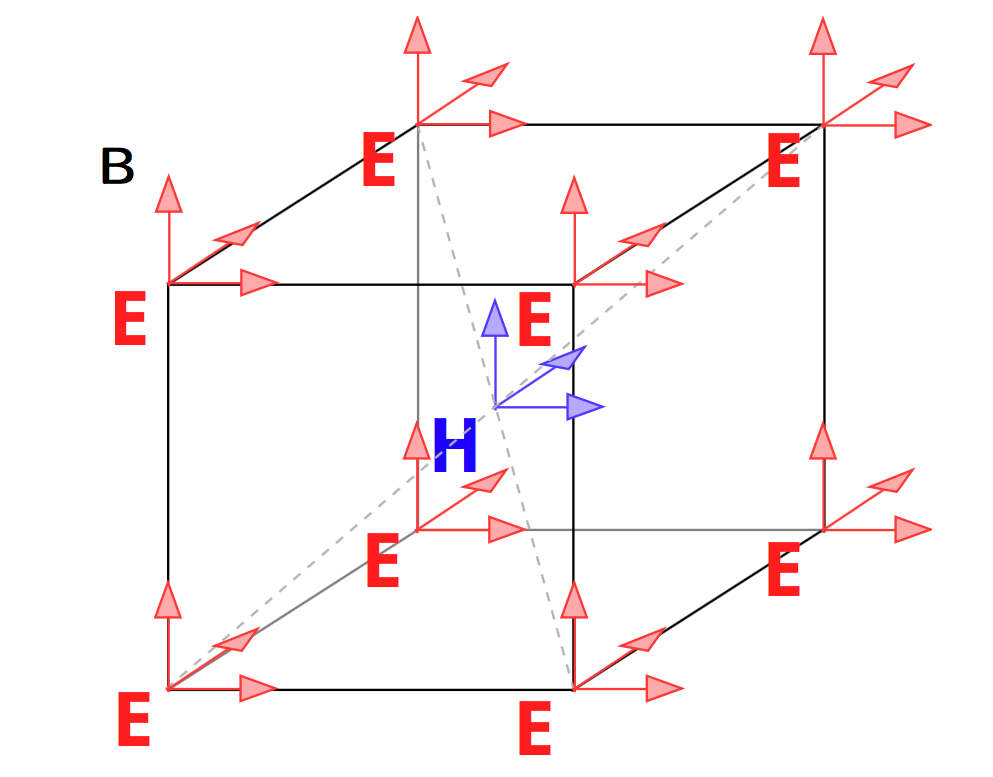
\includegraphics[width=\textwidth]{slike/our_lattice_fields.png}
	\phantomcaption
	\label{fig:ourlatticefields}
	\end{subfigure}\quad
	\begin{subfigure}[b]{0.45\textwidth}
	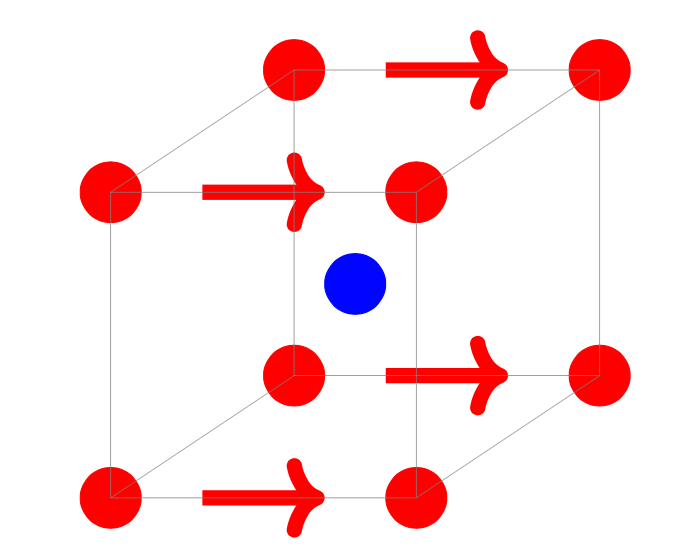
\includegraphics[width=\textwidth]{slike/our_lattice_derivatives.png}
	\phantomcaption
	\label{fig:ourlatticederivatives}
	\end{subfigure}
	\caption{\emph{\textbf{a.)} Nadgradnja Yeejeve mreže, ki smo jo uporabljali v naši implementaciji metode FDTD. Slika prikazuje, da čeprav položaji točk ostajajo enaki, so za razliko od Yeejeve mreže tu vse komponente polj shranjene v vsaki točki. \textbf{b.)} Primer izračuna $\partial \mathbf{E}/\partial x$. Z rdečimi pikami so označeni položaji kjer je shranjen $\mathbf{E}$, s puščicami kjer so izračunani posamezni odvodi po $x$, z modro piko pa mesto kjer odvod zares potrebujemo in kjer je definiran $\mathbf{H}$. Vir slik: \cite{cancula}}}
\end{figure}

Ker imamo sedaj vse komponente polja v vseh točkah, je potrebno prilagoditi računanje krajevnih odvodov. Slika \ref{fig:ourlatticederivatives} s puščicami prikazuje mesta, kjer je izračunan odvod $\partial \mathbf{E}/\partial x$. Mesto, kjer ta odvod potrebujemo, je označeno z modro piko, kjer je definirano magnetno polje $\mathbf{H}$. V vsakem koraku, tako za $\partial \mathbf{E}/\partial x$ 
vzamemo povprečje odvodov označenih s puščicami. Podrobno je postopek izračuna odvodov v naši implementaciji razložen v Dodatku ...

\subsection{Izvori valovanja in robni pogoji}

V splošnem, Maxwellove enačbe vsebujejo izvore elektromagnetnih polj. Vendar za primere modeliranja toka svetlobe skozi materiale le redko potrebujemo izvore valovanja znotraj simulacijske celice. Ponavadi nas bolj zanimajo primeri v katerih svetloba (svetlobni snop, svetlobni pulz, ...) vpada na simulacijsko celico od zunaj. Podobno pa, ko vpadna svetloba prepotuje našo celico, želimo, da se vanjo ne vrne v obliki odboja. Oboje je v simulaciji moč doseči z izrabo posebnih robnih pogojev ter uvedbo dodatnih plasti okoli celice.\\

Izvor valovanja v simulacijo vpeljemo tako, da okoli celice dodamo namišljeno \emph{mejno plast} (\emph{boundary layer}) veliko manjše debeilne kot je velikost celice. Med simulacijo v vsaki iteraciji na meji med plastjo in celico prištejemo ali odštejemo ustrezno električno ali magnetno polje želenega izvora, ko računamo končne diference med točko v celici in točko v mejni plasti. \\

Absorpcijo svetlobe, ko svetloba prepotuje simulacijsko celico, lahko prav tako zagotovimo z vpeljavo še ene plasti v kateri velja Beer-Lambertov absorpcijski zakon\cite{beerlambert}. Žal pa je takšna absorpcija za metodo FDTD prepočasna, saj mora svetloba prepotovati vsaj nekaj valovnih dolžin preden se popolnoma absorbira, kar močno poveča simulacijsko celico. Poleg tega moramo, če se želimo izogniti odbojem na meji med materialoma, absorpcijski koefecient počasi večati, kar bi še dodatno povečalo celico in s tem podaljšalo računski čas. Rešitev tega problema, je pred dobrima dvema desetletjema ponudil Berenger\cite{berenger}. Ideja predvideva vpeljavo t.i. sloja s popolnim ujemanjem -- PML (\emph{perfectly matched layer}). Električna ($\sigma$) ter (nefizikalna) magnetna ($\sigma_m$) prevodnost v njem prispevata člena $\sigma \mathbf{E}$ ter $\sigma_m \mathbf{H}$ enačbama (\ref{maxwelldiscrete}). Če se za trenutek vrnemo na enodimenzionalni problem in zapišemo enačbe prepuščenega in odbitega valovanja vpadlega na mejo med simulacijsko celico ($\sigma = \sigma_m = 0$) ter absorptivno plastjo ($\sigma$, $\sigma_m$) dobimo izraza za \emph{prepustnost} $T$ ter \emph{odbojnost} $R$ takšne meje
\begin{equation}
T = \frac{2\eta_2}{\eta_1+ \eta_2} \qquad \Gamma = \frac{\eta_2 - \eta_1}{\eta_2 + \eta_1},
\end{equation}
kjer je $\eta_i$ določen z lastnostmi obeh materialov
\begin{equation}
\eta_i = \frac{\mu_i \left (1-\I\frac{\sigma_{mi}}{\omega \mu_i}\right )}{\varepsilon_i \left (1-\I \frac{\sigma_i}{\omega \varepsilon_i} \right )}.
\end{equation}
Vidimo, da obstaja pogoj $\eta_1 = \eta_2$, ko $\Gamma = 0$ in ne pride do odboja! Pri simulacijah v eni dimenziji, se odbojem od mejne plasti izognemo tako, da pravilno izberemo $\mu_2$ ter $\varepsilon_2$ skupaj z ustreznima $\sigma$ ter $\sigma_m$. Žal pa je tako ujemanje mogoče zgolj v eni dimenziji, ko je valovni vektor svetlobe vedno pravokoten na mejo med sredstvoma. V treh dimenzijah pa so na primer v primeru svetlobnih snopov, prisotni tudi ostali vpadni koti. V primeru poljubnega vpadnega kota lahko vsako komponento polja zapišemo kot skalarno vsoto dveh podkomponent, pripadajočih smeri širjenja. Na primer v dvodimenzionalnem primeru je lahko $\mathbf{k} = (k_x, k_y, 0)$, $\mathbf{E} = (E_x, E_y, 0)$ ter $\mathbf{H} = (0,0,H_z)$. Sedaj \emph{razdelimo} (\emph{split}) komponento $H_z$ 
\begin{equation}
\qquad H_z = H_{zx} + H_{zy},
\end{equation}
kjer $H_{zx}$ pripada komponenti valovanja, ki se širi s $k_x$, $H_{zy}$ pa tisti s $k_y$.
Če sedaj vsaki komponenti pripišemo drugačen $\sigma_x$ oziroma $\sigma_y$ ($\sigma_{mx}$, $\sigma_{my}$) in to upoštevamo v sedaj štirih enačbah lahko zagotovimo ujemanje plasti za vse vpadne kote. Transverzalna komponenta valovanja se namreč po vpadu propagira po mejni plasti, dokler ne doseže mejne plasti na katero vpade pravokotno in se absorbira takrat. Na ta način ustvarimo plast s katero lahko absorbiramo vso vpadlo svetlobo. V praksi zaradi diskretizacije prostora še zmeraj pride do odbojev. Teh je manj, če postavimo $\sigma = \sigma(x) \propto x^2$, torej da počasi vključujemo prevodnost materiala.

\subsection{Stabilnost}

Diskretizacija prostora povzroči \emph{numerično disperzijo} valovanja. Običajna disperzijska relacija, za valovanje s frekvenco $\omega$, hitrostjo $c$ in valovnim vektorjem $\mathbf{k}$ je
\begin{equation}
\left ( \frac{\omega}{c} \right )^2 = k_x^2 + k_y^2 +k_z^2.
\label{dispersionrelation}
\end{equation}
Ob diskretizaciji mreže, pa se ta relacija spremeni. Kot je moč pokazati velja,
\begin{equation}
\left [\frac{1}{c\Delta_t} \sin \left (\frac{\omega \Delta_t}{2} \right ) \right ]^2 = \left [\frac{1}{\Delta_x} \sin \left (\frac{k_x \Delta_x}{2} \right ) \right ]^2 + \left [\frac{1}{\Delta_y} \sin \left (\frac{k_y \Delta_y}{2} \right ) \right ]^2 + \left [\frac{1}{\Delta_z} \sin \left (\frac{k_z \Delta_z}{2} \right ) \right ]^2.
\label{numdispersion}
\end{equation}
Ta relacija preide nazaj v (\ref{dispersionrelation}), ko $\Delta_i \rightarrow 0$. Napako v fazi $\phi_{error}$, ki jo pridobi propagirana svetloba na svoji poti dolžine $d$ zaradi diskretizacije definiramo kot
\begin{equation}
\phi_{napaka} = (\tilde{k} - k)d.
\end{equation}
Tu je $\tilde{k}$ valovno število v diskretnem primeru za katerega velja numerična disperzijska relacija (\ref{numdispersion}), $k$ pa valovno število v zveznem primeru. Enačba (\ref{numdispersion}) pravzaprav pomeni močno anizotropijo torej odvisnost fazne napake od smeri propagacije (vektorja $\mathbf{\tilde{k}}$). Amplituda fazne napake je določena z velikostjo krajevnih korakov $\Delta_i$. Slika \ref{fig:phaseerror3D} prikazuje fazno napako pridobljeno s prepotovano valovno dolžino $\lambda$ pri diskretizaciji mreže $\Delta = \Delta_x = \Delta_y = \Delta_z = \lambda/20$. Na Sliki \ref{fig:phaseerrorazimuthal} pa je prikazana zgolj odvisnost fazne napake pri $z=0$ za azimutalni kot $\varphi$ v tej ravnini pri treh različnih vrednostih diskretizacije prostora $\Delta$. Napaka je prikazana v logaritemski skali in jasno prikaže kako hitro se z diskretizacijo zmanjša.

\begin{figure}[h!]
	\centering
	\begin{subfigure}[b]{0.45\textwidth}
	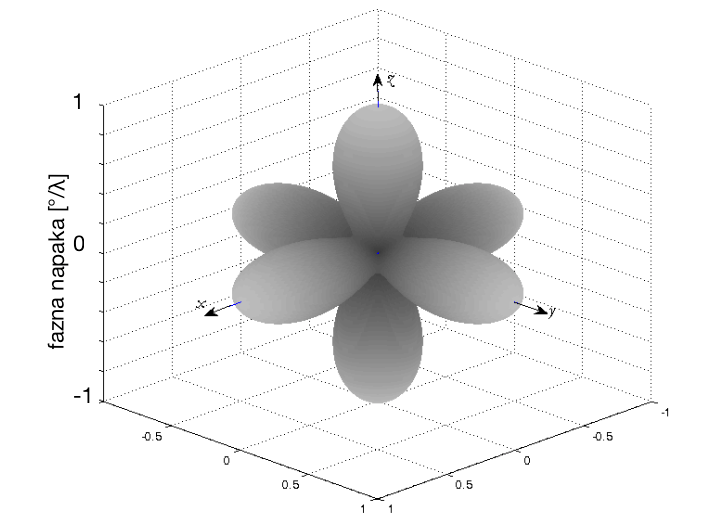
\includegraphics[width=\textwidth]{slike/phase_error_3D.png}
	\phantomcaption
	\label{fig:phaseerror3D}
	\end{subfigure}\quad
	\begin{subfigure}[b]{0.45\textwidth}
	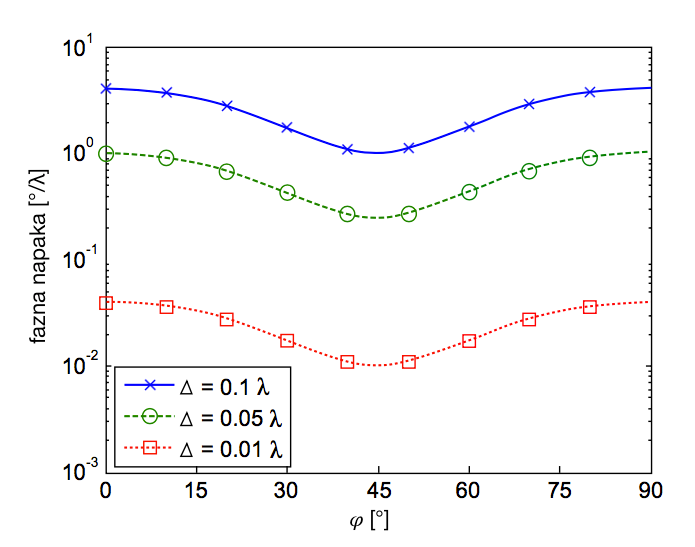
\includegraphics[width=\textwidth]{slike/phase_error_azimuthal.png}
	\phantomcaption
	\label{fig:phaseerrorazimuthal}
	\end{subfigure}
	\caption{\emph{\textbf{a.)} Odvisnost napake v fazi v 3D $k$-prostoru, kjer opazimo, da numerična disperzija pripelje do močne anizotropije. Valovanje, ki se širi vzdolž ene izmed diagonalnih smeri bo na svoji poti pridobilo manjšo napako v fazi kot pa valovanje vzdolž ene izmed glavnih osi. \textbf{b.)} Odvisnost fazne napake od azimutalnega kota za tri različne vrednosti prostorske diskretizacije $\Delta$. Uporabljena je logaritemska skala. Vir slik: \cite{gedney}}}
\end{figure}

Metoda FDTD ni stabilna za poljubno izbiro časovnega ter prostorskega koraka. Enačbo (\ref{numdispersion}) lahko predelamo tako, da dobimo stabilne vrednosti razmerja $\Delta/(c\Delta_t)$. Če enačbo (\ref{numdispersion}) rešimo za $\omega$ dobimo
\begin{equation}
\omega = \frac{2}{\Delta_t}\arcsin(\xi),  
\end{equation}
kjer smo s $\xi$ označili
\begin{equation}
\xi = c\Delta_t \sqrt{ \left [\frac{1}{\Delta_x} \sin \left (\frac{k_x \Delta_x}{2} \right ) \right ]^2 + \left [\frac{1}{\Delta_y} \sin \left (\frac{k_y \Delta_y}{2} \right ) \right ]^2+ \left [\frac{1}{\Delta_z} \sin \left (\frac{k_z \Delta_z}{2} \right ) \right ]^2}.
\end{equation}

Vrednost $\xi$ je omejena navzgor in sicer je največja, ko $k_i\Delta_i/2 = \pm \pi$, kar nam v primeru $\Delta_x = \Delta_y = \Delta_z = \Delta$ da
\begin{equation}
\xi = \frac{c\Delta_t}{\Delta} \sqrt{3}.
\end{equation}
Ker $\omega \propto \arcsin(\xi)$ in je vrednost funkcije $\arcsin(x)$ za $x>1$ \emph{imaginarno število} je pogoj za stabilnost $\xi<1$. To za vrednosti $\Delta_t$ v tem preprostem primeru pomeni
\begin{equation}
c\Delta_t < \frac{\Delta}{\sqrt{3}}.
\end{equation}
Če je časovni korak ali krajevni korak prevelik, je $1 < \xi < \xi_{max}$, ko postaneta $\omega$ ter $k$ imaginarna kar povzroči eksponentno rast ali pojemanje valovanja v simulaciji.

\subsection{Naša implementacija}

Koda za našo implementacijo metode FDTD je napisana deloma v \texttt{Pythonu}, deloma pa v OpenCL in \texttt{C++} programskem jeziku. OpenCL (\emph{Open Computing Language}) je orodje za pisanje kode, ki lahko teče na grafičnih (GPU) ali na procesnih enotah (CPU). Ker v vsakem časovnem koraku posodobimo vse komponente elektromagnetnih polj na celotni mreži je za učinkovitejšo implementacijo metode FDTD moč uporabiti \emph{vzporedno računanje}. Vzporedno računanje je zaradi večjega števila procesnih jeder veliko hitrejše na grafičnih enotah: pri večjih simulacijah, ki smo jih še lahko poganjali na njih je program tekel vsaj 5-krat hitreje. Problem nastane, ko želimo simulirati zares velike celice, saj imajo grafične enote manj spomina kot procesne enote. Zaradi tega je bilo pomembno, da imamo kodo, ki lahko teče v enem ali drugem okolju. \\

V našem primeru smo simulacije najpogosteje poganjali na grafičnih enpotah NVIDIA Titan X, vsaka z 3072 jedri ter 6GB delovnega spomina, kar nam je omogočalo simulacije v celicah velikosti do 50 milijonov točk. Primer celica velikosti $200\times200\times 1300$ z resolucijo $20$nm/piko pomeni prostor velikosti $4\mu \text{m}\times 4\mu \text{m} \times 28 \mu\text{m}$.\\

Pred začetkom simulacije nastavimo vse potrebne parametre
\begin{itemize}
\item{lastnosti celice: velikost v številu pik, resolucija (nm/piko), ...}
\item{dolžina simulacije: število časovnih korakov}
\item{lastnosti vira: valovna dolžina, red Laguerre-Gaussovega snopa, širina snopa, položaj grla, polarizacija, faza,...}
\item{lastnosti snovi: direktorsko polje, izredni in redni lomni količnik, ...}
\end{itemize}
Rezultat simulacije sta seveda polji $\mathbf{E}$ in $\mathbf{H}$ v celotni mreži po vseh pretečenih korakih. Iz njih lahko nadalje izračunamo reprezentativne količine kot je električno polje oziroma intenziteta svetlobe v vseh točkah celice.\\

\chapter{Rezultati}

Osnovni namen tega magistrskega dela je pokazati, da se lahko nematski profil dvojno zvitega cilindra v posebnem primeru, ko nanj vpada azimutalno polarizirana svetloba, obnaša kot leča ali pa kot valovni vodnik. V nadaljevanju bomo predstavili rezultate numeričnih simulacij, opravljenih z metodo FDTD, ki to potrjujejo. \\

To ni prvi primer nematskega profila za katerega je bilo pokazano, da vodi do lečenja in vodenja svetlobe. Podobno se zgodi za radialno polariziran snop, ki vpade na pobegli (\emph{escaped}) nematski profil\cite{cancula,cancula3}.

\section{Lečenje na DTC nematskem profilu}

Vzemimo nematski profil, ki ga opisuje direktor definiran z (\ref{dtcdirector}). Nematske molekule naj bodo anizotropne z razliko lomnih količnikov $\Delta n = n_o - n_e < 0$. Optična os takega profila, torej smer vzdolž katere polarizirana svetloba občuti izredni lomni količnik $n_e$, se enakomerno spreminja v radialni smeri -- v sredini profila ($r=0$) je optična os vzporedna osi cilindra, ob večanju $r$ pa se ne glede na smer oddaljevanja optična os enakomerno suka okoli radialne smeri. Običajno se direktor oziroma optična os v takem profilu zasuka za kot $\pi/4$, lahko pa si zamislimo tudi takšnega, kjer se zasuka za kot $\pi/2$. Ne glede kot zasuka, pa se simetrija takšnega profila ujema z azimutalno polariziranim snopom svetlobe, prikazanim na Sliki \ref{fig:lg_01azimuthalbeam}. V azimutalno polariziranem snopu polarizacija v vsaki točki preseka kaže pravokotno na radialno os, podobno kot ima direktor DTC profila v vsaki točki preseka komponento direktorja prav tako usmerjeno v azimutalni smeri! V vsaki točki preseka je torej kot med optično osjo ter valovnim vektorjem $\mathbf{k}$ enak $\theta$ polarizacija pa je vselej izredna zato je po enačbi (\ref{extraordinaryn}) lomni količnik določen z $n(\theta)$ kot
\begin{equation}
n(\theta) = \frac{n_o n_e}{n_e^2 \sin^2 \theta + n_o^2 \cos^2 \theta}.
\label{dtcrefractiveindex}
\end{equation}
To je prikazano na Sliki \ref{fig:indexellipsoid}, kjer je označena optična os, $\mathbf{k}$ vektor svetlobe ter lastna lomna količnika. Azimutalna polarizacija ima v DTC nematskem profilu vedno komponento vzdolž optične osi zato občuti lomni količnik $n(\theta)$. V DTC profilu se kot $\theta$ linearno spreminja z $r$ kot
\begin{equation}
\theta(r) = \frac{\pi}{2} (1-q_0\frac{r}{R}),
\end{equation}
kjer je $R$ radij nematskega profila, $q_0$ pa kiralnost, ki določa za kolikšen kot se direktor zasuka do $r = R$. Če imamo opisani profil v nematiku z negativno dvolomnostjo ko je $\Delta n < 0$ oziroma $n_e < n_o$ ima lomni količnik (\ref{dtcrefractiveindex}) obliko prikazano na Sliki \ref{fig:dtcrefractiveindex3d}. V prikazanem primeru je $n_e = 1.50$, $n_o = 1.45$ ter $\Delta n = -0.05$.

\begin{figure}[h!]
	\centering
	\begin{subfigure}[b]{0.25\textwidth}
	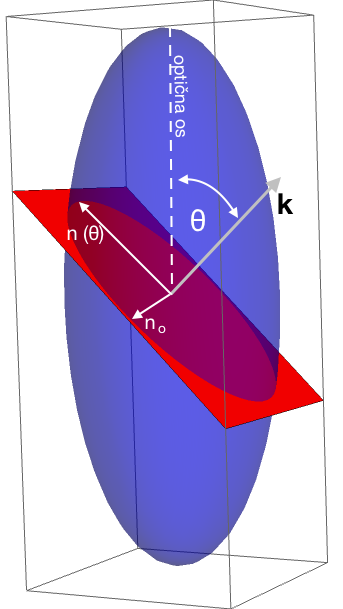
\includegraphics[width=\textwidth]{slike/ellipsoid.png}
	\phantomcaption
	\label{fig:indexellipsoid}
	\end{subfigure}\qquad
	\begin{subfigure}[b]{0.55\textwidth}
	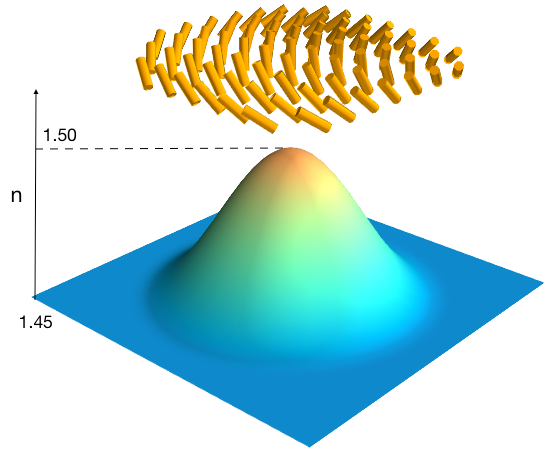
\includegraphics[width=\textwidth]{slike/nematic_refractive_xyz.png}
	\phantomcaption
	\label{fig:dtcrefractiveindex3d}
	\end{subfigure}
	\caption{\emph{\textbf{a.)} Elipsoid z dolžinama polosi $n_e$ ter $n_o$, kjer $n_o<n_e$, ter valovni vektor $\mathbf{k}$ svetlobe, ki predstavlja smer v kateri svetloba potuje, ter skupaj s polarizacijo določa lomni količnik. \textbf{b.)} Odvisnost lomnega količnika v preseku dvojno zvitega cilindra za negativno dvolomen nematik. Prikazana je tudi ena plast DTC profila.}}
\end{figure}

Faza, ki jo pridobi svetloba, ki se giblje skozi plast snovi debeline $d$ z lomnim količnikom $n$ je enaka $\phi = nd$. Prikazani profil lomnega količnika povzroči, da azimutalno polariziran snop doživi večji fazni zamik v centru DTC profila kot na robovih, kjer je lomni količnik manjši! To je čisto analogno  situaciji ob vpadu svetlobe na običajno zbiralno lečo. Zbiralna steklena leča s konstantnim lomnim količnikom $n_{stekla} = 1.458$ je oblikovana tako, da je debelejša na sredini in tanjša ob robovih, kar pomeni, da bo fazni zamik ob osi leče kot proč od nje. Enačba, ki opisuje fazni zamik v bikonveksnih lečah v približku tanke leče je
\begin{equation}
\Delta \phi = \frac{2\pi}{\lambda} \frac{r^2}{2f},
\end{equation}
kjer je $f$ goriščna razdalja leče (določena s krivinskima radijema obeh površin), $r$ razdalja od osi leče, $\lambda$ pa valovna dolžina vpadne svetlobe. Fazna zamika v obeh primerih lahko primerjamo, kar je prikazano na Sliki \ref{fig:phaseshiftcomp} za primer $d = 15$ $\mu$m ter $f = 20$ $\mu$m.\\

\begin{figure}[h!]
	\centering
	\begin{subfigure}[b]{0.7\textwidth}
	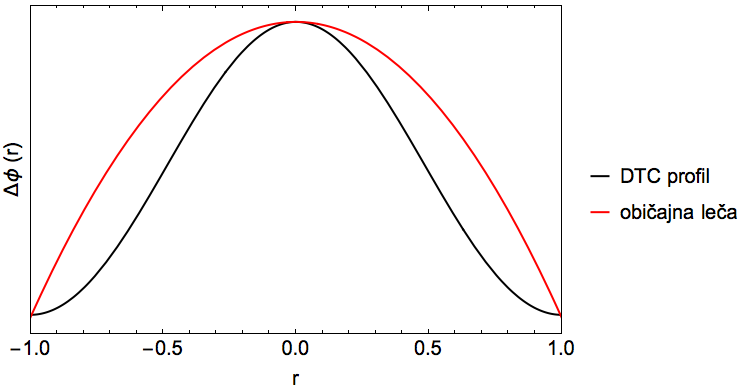
\includegraphics[width=\textwidth]{slike/phase_shift_comparisson.png}
	\end{subfigure}
	\label{fig:phaseshiftcomp}
	\caption{\emph{Primerjava faznega zamika, ki ga povzroči običajna steklena leča v primerjavi z zamikom, ki ga na azimutalno polariziranem snopu, povzroči DTC profil debeline $d$.}}
\end{figure}

Začetne numerične simulacije lečenja z metodo FDTD so bile opravljene z lastnostmi simulacijske celice in parametri žarka ter nematskega profila predstavljenimi v Tabeli \ref{lensingparameters1}.
\begin{table}[h!]
\centering
\caption{\emph{Lastnosti celice, žarka ter nematskega profila uporabljene v osnovnih simulacijah lečenja na DTC nematskem profilu.}}
\label{lensingparameters1}
\begin{tabular}{ll}
\hline
\multicolumn{1}{|l|}{velikost celice}  & \multicolumn{1}{l|}{$240 \times 240 \times 1000$} \\ \hline
\multicolumn{1}{|l|}{resolucija}       & \multicolumn{1}{l|}{30 nm/vox}        \\ \hline
\multicolumn{1}{|l|}{debelina DTC} & \multicolumn{1}{l|}{250 vox}          \\ \hline
\multicolumn{1}{|l|}{radij DTC}    & \multicolumn{1}{l|}{110 vox}          \\ \hline                     
\end{tabular}\quad
\begin{tabular}{ll}
\hline
\multicolumn{1}{|l|}{kiralnost, $q_0$}    & \multicolumn{1}{l|}{1.0}          \\ \hline   
\multicolumn{1}{|l|}{$n_o$, $n_e$}  & \multicolumn{1}{l|}{1.45, 1.50} \\ \hline
\multicolumn{1}{|l|}{vpadna polarizacija}       & \multicolumn{1}{l|}{azimutalna}        \\ \hline
\multicolumn{1}{|l|}{valovna dolžina, $\lambda$} & \multicolumn{1}{l|}{400 nm}          \\ \hline                  
\end{tabular}
\end{table}

Celica je oblike poldogovatega kvadra in daljše stranice ustrezajo smeri osi cilindra ter smeri propagacije svetlobe. Parameter, ki se je spreminjal v teh začetnih simulacijah je bila vstopna širina žarka $w_0$.  Vstopni žarek je imel v vseh primerih Laguerre-Gaussov amplitudni profil (enačba \ref{laguerregaussianamplitude}), reda ($p=0$, $\ell = 1$) in tak, da je imel grlo na mestu vstopa v simulacijsko celico torej tudi na mestu, kjer se je začel nematski DTC profil. Kako močan je fazni zamik določa debelina profila $d$ ter dvolomnost molekul $\Delta n$. Po propagaciji skozi DTC profil preide svetloba v območje, kjer je definiran uniformen nematski profil z usmerjenostjo v smeri osi $z$. Rezultati opisanih simulacij so prikazani na Sliki \ref{fig:lensingresults1}.

\begin{figure}[h!]
	\centering
	\begin{subfigure}[b]{1\textwidth}
	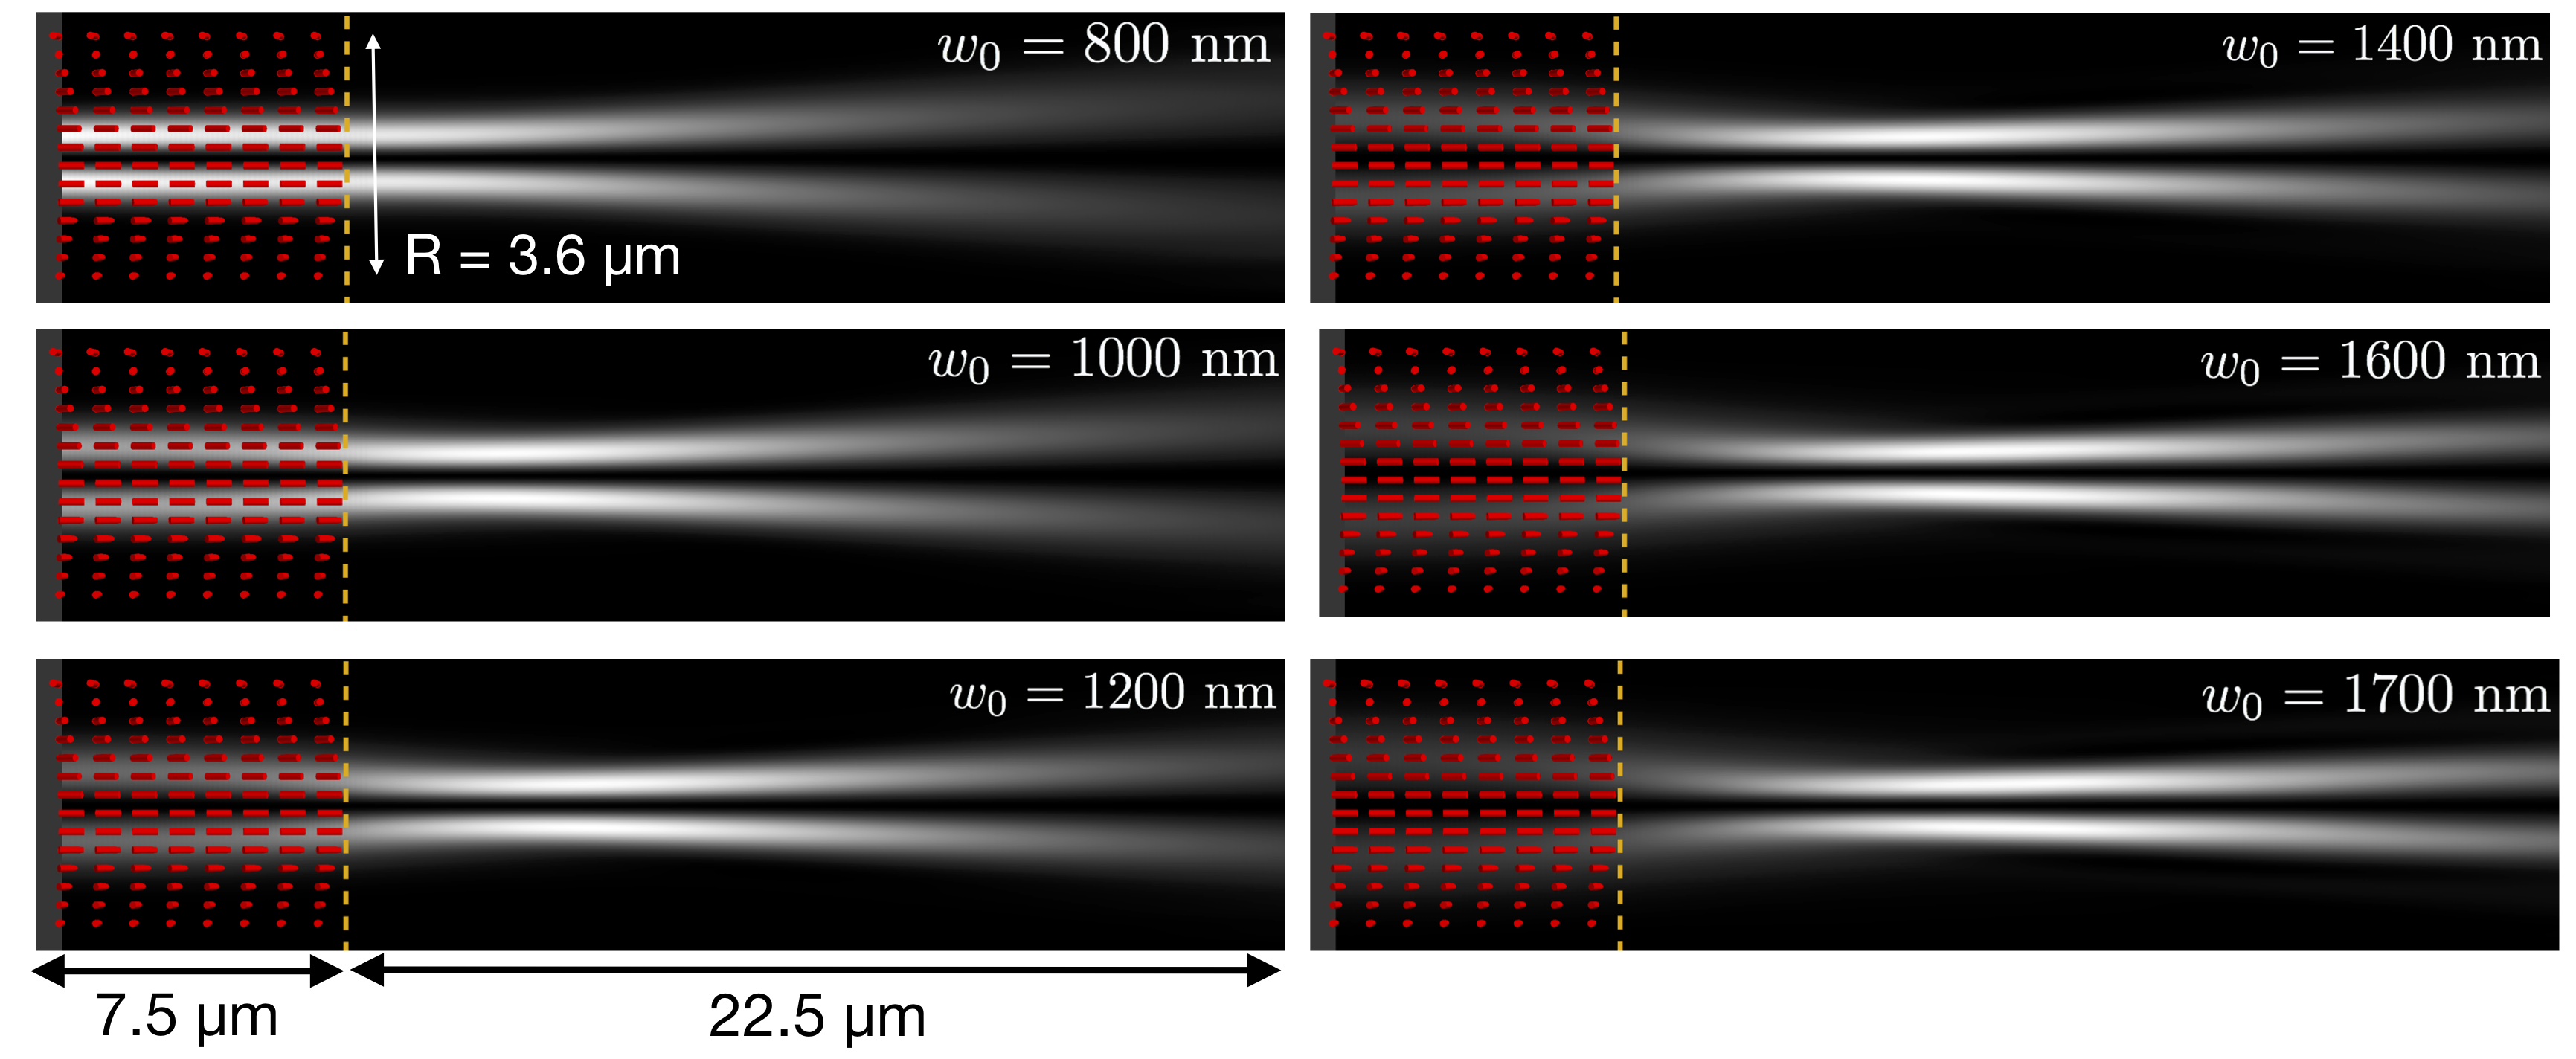
\includegraphics[width=\textwidth]{slike/lensing_31_5.png}
	\end{subfigure}
	\caption{\emph{Simulacije lečenja svetlobe na DTC nematskem profilu debeilne $ d = 7.5$ $\mu$m za različne vstopne širine snopa $w_0$. Prikazani so $yz$ prerezi v sredini snopa, svetloba pa na vseh slikah potuje v desno, v smeri osi $z$.}}
	\label{fig:lensingresults1}
\end{figure}

Vidimo, da postaja lečenje vse močnejše s širino vpadnega snopa, kajti ta vse bolj vpada na območje DTC profila kjer se $n$ najbolj hitro spreminja zato različni deli žarka pridobijo večjo medsebojno fazno razliko. Zanimivo si je ogledati tudi kakšna je širina žarkov vzdolž osi $z$ za različne vstopne širine, kar iz zgornje slike ne opazimo zlahka. Iz takšnih profilov lahko izloščimo tudi položaj in širino grla snopa po prehodu skozi DTC lečo. Za tri različne vstopne širine $w_0$, je to prikazano na Sliki \ref{fig:widthprofiles1} za dve različni debelini leč $d$. 

\begin{figure}[h!]
	\centering
	\begin{subfigure}[b]{0.6\textwidth}
	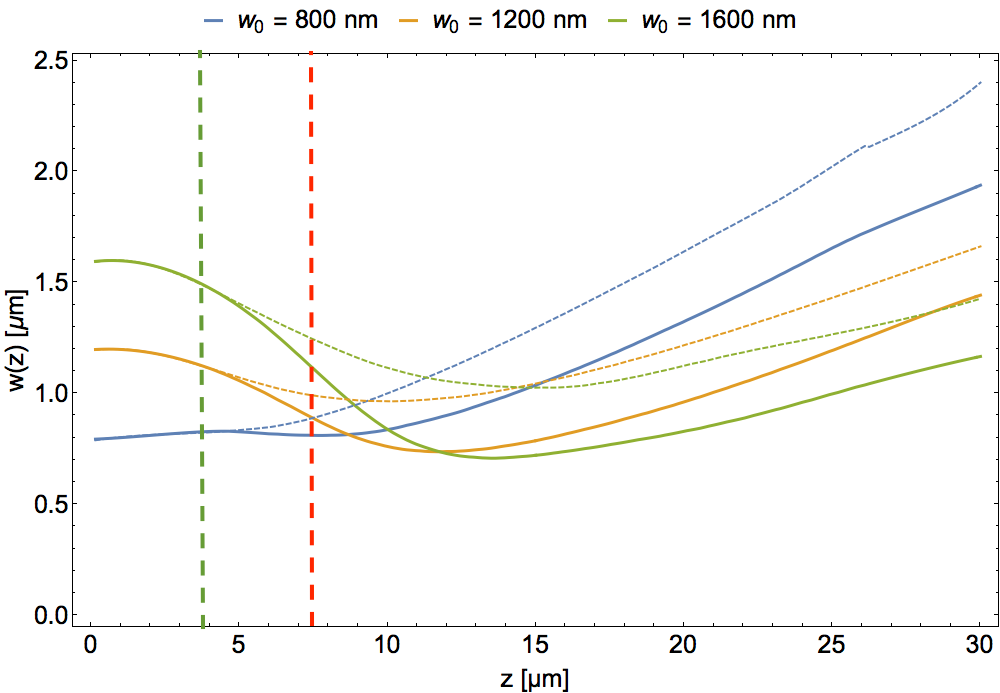
\includegraphics[width=\textwidth]{slike/width_profiles_2.png}
	\end{subfigure}
	\label{fig:widthprofiles1}
	\caption{\emph{Profili širine treh snopov z različno vstopno širino vzdolž osi $z$. Položaja, kjer se končata DTC nematska profila debelin $d = 3.75$ $\mu$m ter $d = 7.5$ $\mu$m sta označena z zeleno in rdečo navpično črtkano črto.}}
\end{figure}
Opazimo, da se lečenje prične že znotraj nematskega profila za večje vstopne širine pa se grlo snopa oddaljuje od leče in postaja ožje.\\

Radialno polariziran snop še na gornjo sliko!\\

\subsection{Cilindrično lečenje}

Spremembe polarizacije, simulacije 14.3!

\section{Vodenje svetlobe}

Opisano lečenje na DTC nematskem profilu je moč razširiti na vodenje svetlobe, ki ga poznamo v optičnih vlaknih. Še več, ker radialno polarizirana svetloba ne občuti spreminjanja lomnega količnika je ni moč voditi po DTC proflu, kar pomeni, da lahko takšen profil deluje kot polarizacijsko občutljivi valovni vodnik, ki deluje le za pravilno izbrano vstopno polarizacijo.

\subsection{Vodenje svetlobe v zakrivljenem profilu}

Zanimalo nas je tudi, če je mogoče tak profil zakriviti, vsaj v eni dimenziji in kakšne posledice ima to za izgube v valovnem vodniku. Takšen profil smo modelirali kot del krožnice s krivinskim radijem $R_k$. Direktor v središču zakrivljenega dvojno-zvitega cilindra seveda sledi zakrivljenosti osi.

\section{Vodenje svetlobe v modrih fazah}

Kot omenjeno v poglavju o modrih fazah, so dvojno-zviti cilindri gradniki v modrih fazah naloženi v pravilno preprosto kubično ali ploskovno centrirano kubično rešetko. Osnovni celici modrih faz tipa 1 in 2 (BP| in BP ||) sta prikazana na Slikah \ref{fig:bp1} ter \ref{fig:bp2}. Iz numeričnih izračunov tenzorja ureditvenega parametra osnovnih celic v modrih fazah, opravljenih z metodo opisano v \cite{ravnik,ravnik3}, smo lahko prišli do direktorskega profila v eni osnovni celici. Za prikaz smo vzeli osnovno celico BP2 in sestavili več takšnih celic skupaj tako, da smo sestavili daljši dvojno-zviti cilinder, ki je sedaj del modrih faz. Tak direktorski profil ni več čisti DTC profil, ki smo ga opisovali do sedaj, saj se periodično srečuje z ostalimi cilindri, kar povzroči lokalno spreminjanje direktorja na robu. To ima posledice za lomni količnik za azimutalno polarizirano vpadno svetlobo, za katero se sedaj vzdolž osi $z$ poravnane z osjo sestavljenega cilindra, ta vzdolž osi $z$ spreminja, kot je prikazano na Sliki \ref{fig:bluephaseindex}.
\begin{figure}[h!]
	\centering
	\begin{subfigure}[b]{0.9\textwidth}
	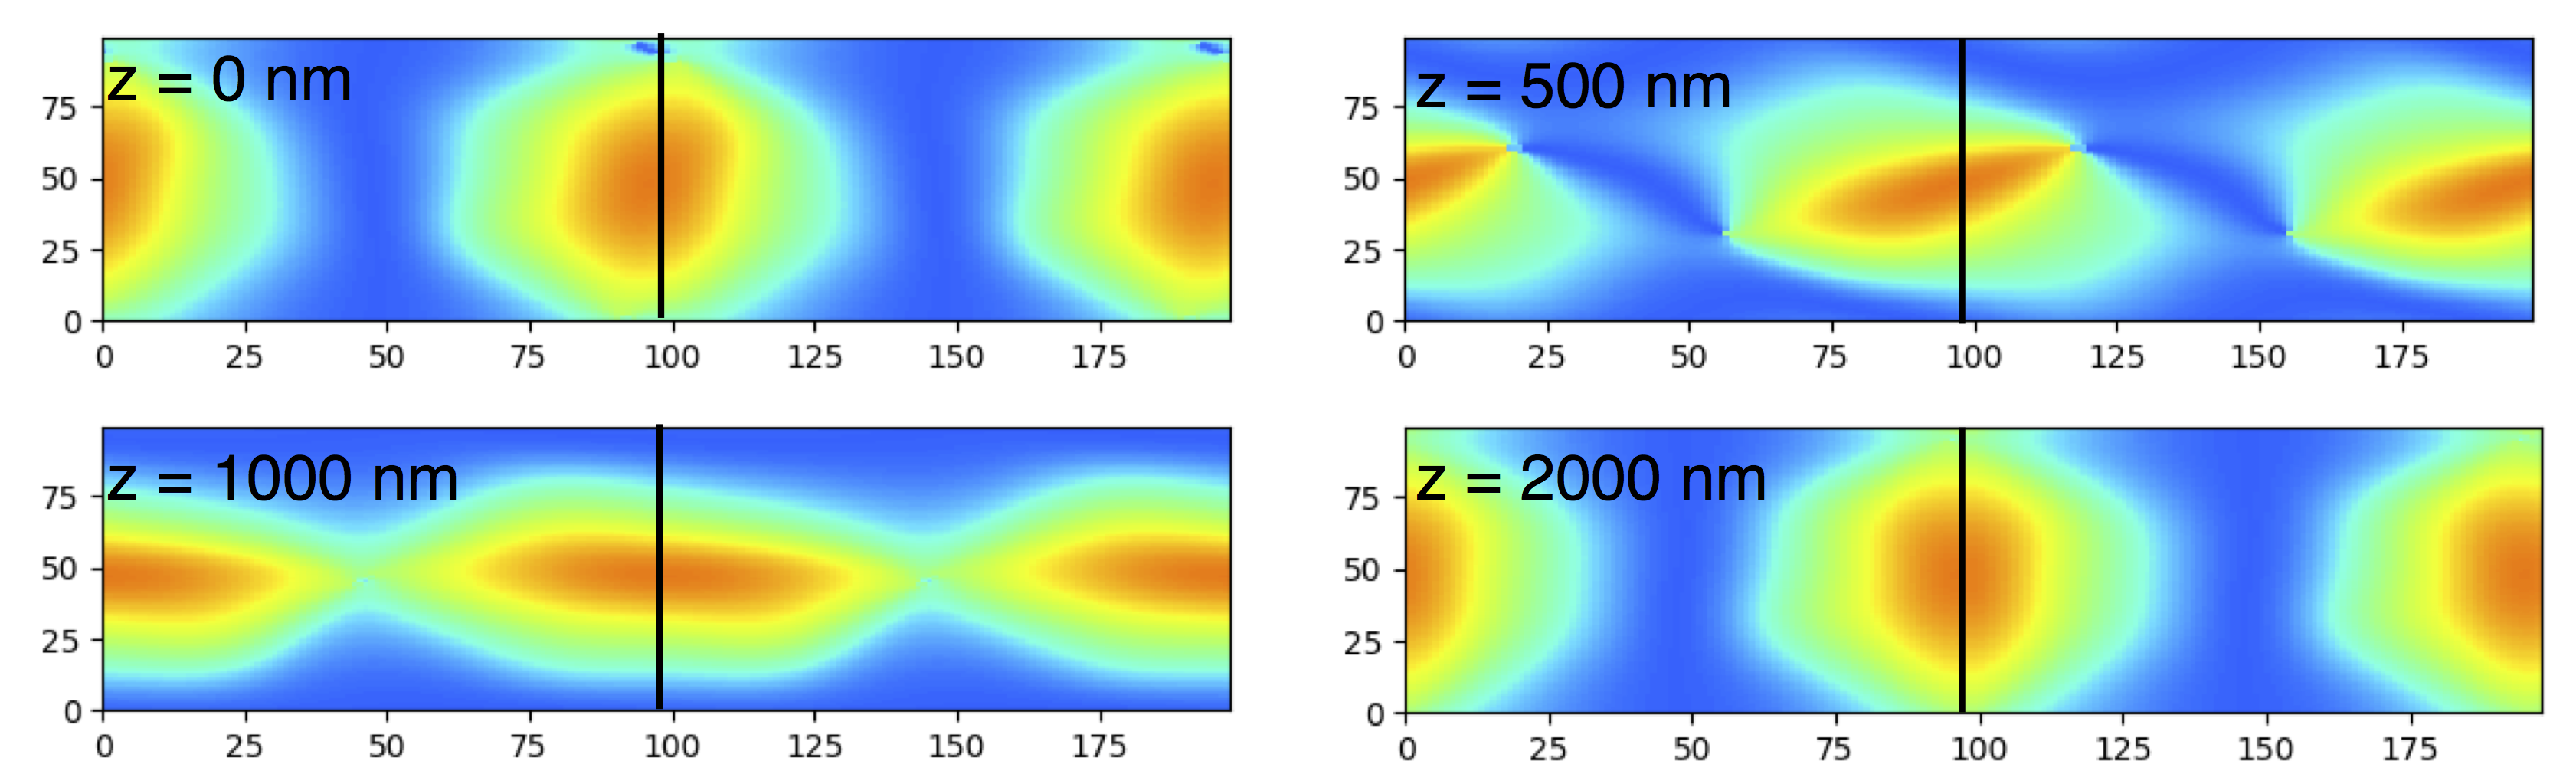
\includegraphics[width=\textwidth]{slike/bp_n.png}
	\end{subfigure}
	\label{fig:bluephaseindex}
	\caption{\emph{Spreminjanje profila lomnega količnika vzdolž osnovne celice v $z$ smeri. S črno črto na sredini, je označeno mesto, kjer smo združili dve osnovni celici BPII.}}
\end{figure}
 
%%%%-------------------ZAKLJUČEK-------------------------%%%%%
\chapter{Zaključek}


%%% LITERATURA

\cleardoublepage\phantomsection
\addcontentsline{toc}{chapter}{Literatura}
\bibliographystyle{myapsrevSLO}

%------------------------BIBLIOGRAFIJA------------------------%
\bibliography{Bibliografija}
\begin{thebibliography}{15}
%-------UVOD----------%
\bibitem{willner}
	A. E. Willner, R. L. Byer, \emph{et. al.},
	\emph{Optics and Photonics: Key Enabling Technologies},
	Proce. of the IEEE, (\textbf{100}), 1604-1634, 2012.
	
\bibitem{abbott}
	B. P. Abbott \emph{et. al.},
	\emph{Observation of Gravitational Waves from a Binary Black Hole Merger},
	Phys. Rev. Lett., \textbf{116}, 2016.
	
\bibitem{klar}
	T. A. Klar, S. W. Hell,
	\emph{Subdiffraction resolution in far-field fluorescence microscopy},
	Opt. Lett., (\textbf{24}), 954-956, 1999.
	
\bibitem{mikami}
	H. Mikami, L. Gao, K. Goda,
	\emph{Ultrafast optical imaging technology: principles and applications of emerging methods},
	Nanophotonics, (\textbf{5}), 497-509, 2016.
	
\bibitem{soukolis}
	C. M. Soukolis, M. Wegener, 
	\emph{Past achievements and future challenges of three-dimensional photonic metamaterials},
	Nat. Phot., (\textbf{5}), 523-530, 2011.

\bibitem{jahani}
	S. Jahani, Z. Jacob, 
	\emph{All-dielectric metamaterials},
	Nat. Nanotech., (\textbf{11}), 23-36, 2016.
	
\bibitem{shelby}
	R. A. Shelby, D. R. Smith, S. Schultz,
	\emph{Experimental verification of a negative index of refraction},
	Science, (\textbf{292}), 77-79, 2001.

\bibitem{pendry}
	J. B. Pendry, D. Schurig, D. R. Smith,
	\emph{Controlling electromagnetic fields},
	Science, (\textbf{312}), 1780-1782, 2006.

\bibitem{ergin}
	T. Ergin, N. Stenger, P. Brenner, J. B. Pendry, M. Wegener
	\emph{Three-dimensional invisibility cloak at optical wavelengths},
	Science, (\textbf{328}), 337-339, 2010.

\bibitem{siliconphotonics}
	\emph{Silicon Photonics} [focus issue],
	Nat. Phot., (\textbf{4}), 491-578, 2011.

\bibitem{siliconphotonicsintel}
	\url{http://www.intel.com/content/www/us/en/architecture-and-technology/silicon-photonics/silicon-photonics-overview.html}, dostopano: 24. 5. 2017.

\bibitem{bose}
	R. Bose, D. Sridharan, H. Kim, G. S. Solomon, E. Waks, 
	\emph{Low-photon number optical switching with a single quantum dot coupled to a photonic crystal cavity},
	Phys. Rev. Lett., (\textbf{108}), 227402, 2012.

\bibitem{espinosa}
	T. Espinosa-Ortega, T. C. H. Liew,
	\emph{Complete architecture of integrated photonic circuits based on and not and not logic gates of exciton polaritons in semiconductor microcavities},
	Phys. Rev. B, (\textbf{87}), 195305, 2013.

\bibitem{chen}
	W. Chen, K. M. Beck, R. Bücker, M. Gullans, M. D. Lukin, H. Tanji-Suzuku, V. Vuletić,
	\emph{All-optical switch and transistor gated by one stored photon},
	Science, 768-770, 2013.
	
\bibitem{musevic}
	I. Muševič,
	\emph{Liquid-crystal micro-photonics},
	Liq. Crys. Rev., (\textbf{4}), 1-34, 2016.

\bibitem{yeh}
	P. Yeh, C. Gu, 
	\emph{Optics of liquid crystal displays},
	Wiley, 2010.

\bibitem{coles2}
	H. Coles, S. Morris,
	\emph{Liquid-crystal lasers},
	Nat. Phot, (\textbf{4}), 676-685, 2010.

\bibitem{cancula}
	M. Čančula.
	\emph{Mutually coupled flow of light and liquid crystal ordering} (doktorska disertacija),
	FMF, Ljubljana, 2017.
	
\bibitem{saleh}
	B. E. A. Saleh, M. C. Teich.
	\emph{Fundamentals of photonics},
	Wiley, New Jersey (NJ), 2007.
	
\bibitem{podgornik}
	R. Podgornik, A. Vilfan,
	\emph{Elektromagnetno polje},
	DMFA, Ljubljana, 2012.



%------VECTOR BEAMS-------%
\bibitem{zhan}
	Q. Zhan,
	\emph{Cylindrical vector beams: from mathematical concepts to applications},
	Adv. Opt. Photonics, \textbf{1}, 1-57 (2009).

\bibitem{dorn}
	R. Dorn, S. Quabis, G. Leuchs,
	\emph{Sharper focus for a radially polarized light beam},
	Phy. Rev. Lett., \textbf{91}, 23, 2003.
	
\bibitem{niziev}
	V. G. Niziev, A. V. Nesterov,
	\emph{Influence of beam polarization on laser cutting efficiency},
	Jour. of Physics D, (\textbf{32}), 13, 1999.

\bibitem{youngworth}
	K. S. Youngworth, T. G. Brown,
	\emph{Focusing of high numerical aperture cylindrical-vector beams},
	Opt. Express, (\textbf{7}), 77-87, 2000.
	
\bibitem{kozawa}
	Y. Kozawa, S. Sato,
	\emph{Generation of radially polarized laser beam by use of a conical Brewster prism},
	Opt. Letters, (\textbf{30}), 3063-3065, 2005.

\bibitem{volpe}
	G. Volpe, D. Petrov,
	\emph{Generation of cylindrical vector beams with few-mode fibers excited by Laguerre–Gaussian beams},
	Opt. Comm., (\textbf{237}), 89-95, 2004.
	
\bibitem{ko}
	S. Ko, C. Ting, A. Fuh, T. Lin,
	\emph{Polarization converters based on axially symmetric twisted nematic liquid crystal},
	Opt. Express, (\textbf{18}), 3601-3607, 2010.

\bibitem{cancula2}
	M. Čančula, M. Ravnik, S. Žumer,
	\emph{Generation of vector beams with liquid crystal disclinations lines},
	Phy. Rev. E, (\textbf{90}), 2, 2014. 

%------LIQUID CRYTALS
\bibitem{degennes}
	P. G. de Gennes, J. Prost,
	\emph{The Physics of Liquid Crystals},
	Clarendon Press, Oxford, 1993.
	
\bibitem{collings}
	P. J. Collings, M. Hird,
	\emph{Introduction to Liquid Crystals: Chemistry and Physics},
	Taylor\&Francis, 1997.
	
\bibitem{chandrasekhar}
	S. Chandrasekhar
	\emph{Liquid Crystals},
	Cambridge University Press, 1992.
	
\bibitem{gramsbergen}
	E. F. Gramsbergen, L. loNGA, W. H. de Jeu,
	\emph{Landau theory of the nematic-isotropic phase transition}
	Phy. Rep., \textbf{135}, 195-257, 1986.
	
\bibitem{liquidcrystaltypes}
	TCI America,
	\emph{Liquid crystal (LC) materials},
	\url{http://www.tcichemicals.com/eshop/en/us/category_index/12775/}, dostop: 2. 5. 2017.

\bibitem{ravnik}
	M. Ravnik, S. Žumer,
	\emph{Landau-de Gennes modelling of nematic liquid crystal colloids},
	Liq. Crys., \textbf{36}, 1201-1214.
	
\bibitem{lavrenovitch}
	D. Kleman, O. D. Lavrenovitch,
	\emph{Soft Matter Physics: An Introdution},
	Springer, New York, 2003.

\bibitem{cardano}
	F. Cardano, E. Karimi, S. Slussarenko, L. Marucci, C. de Lisio, E. Santamato,
	\emph{Polarizaiton pattern of vector vortex beams generated by q-plates with different topological charges},
	Appl. Optics, (\textbf{51}), C1-C6, 2012.
	
\bibitem{marrucci}
	L. Marrucci, C. Manzo, D. Paparo,
	\emph{Optical spin-to-orbital angular momentum conversion in inhomogeneous anisotropic media},
	Phys. Rev. Lett., (\textbf{96}), 16, 2006.

%BLUE PHASES
\bibitem{wright}
	D. C. Wright, N. D. Mermin,
	\emph{Crystalline liquids: the blue phases},
	Rev. Mod. Phys., \textbf{61}, 385-432, 1989.

\bibitem{kikuchi}
	H. Kikuchi, M. Yokota, Y. Hisakado, H. Yang, T. Kajiyama,
	\emph{Polymer-stabilized liquid crystal blue phases}, 
	Nat. Mater., (\textbf{1}), 64-68, 2002.

\bibitem{coles}
	H. J. Coles, M. N. Pivnenko,
	\emph{Liquid crystal `blue phases' with a wide temperature range}, 
	Nature, (\textbf{436}), 997-1000, 2005.

\bibitem{ravnik2}
	M. Ravnik, J. Fukuda,
	\emph{Templated blue phases},
	Soft Matter, (\textbf{11}), 8417, 2015.
	
\bibitem{ravnik3}
	M. Ravnik, G. P. Alexander, J. M. Yeomans, S. Žumer,
	\emph{Three-dimensional colloidal crystals in liquid crystalline blue phases},
	PNAS, (\textbf{108}), 5188-5192, 2011.
	
\bibitem{kikuchi2}
	H. Kikuchi, H. Higuchi, Y. Haseba, T. Iwata,
	\emph{Fast electro-optical switching in polymer-stabilized liquid crystalline blue phases for display application},
	SID07 Digest, (\textbf{38}), 1737-1740, 2007.
	
%FDTD REFERENCES%

\bibitem{taflove}
	A. Taflove, S. C. Hagness,
	\emph{Computational electrodynamics. The Finite Difference Time Domain Method},
	Artech House, Norwood (MA), 2005.
	
\bibitem{taflove2}
	A. Taflove, A. Oskooi, S. G. Johnson,
	\emph{Advances in FDTD computational electrodynamics: photonics and nanotechnology},
	Artech house, Norwood(MA), 2013.
	
\bibitem{pedrola}
	G. L. Pedrola
	\emph{Beam propagation method for design of optical waveguide devices},
	Wiley, 2016.	

\bibitem{gedney}
	S. D. Gedney,
	\emph{Introduction to the finite-difference time-domain method for electromagnetics}
	Morgan\&Claypool, 2011.
	
\bibitem{jones}
	R. C. Jones,
	\emph{A new calculus for the treatment of optical systems},
	J. Opt. Soc. Am., \textbf{31}, 488-493 (1941).

\bibitem{lavrinenko}
	A. V. Lavrinenko, J. Lægsgaard, N. Gregersen, F. Schmidt, T. Søndergaard.
	\emph{Numerical Methods in photonics},
	CRC Press, 2015.

\bibitem{berenger}
	 J. P. Berenger, \emph{A perfectly matched layer for the absorption of electromagnetic waves},
	 J. Comput. Phys., \textbf{114}, 185-200, 1994.
	 
\bibitem{schneider}
	J. B. Schneider,
	\emph{Understanding the Finite-Difference Time-Domain Method},
	not published, available at: \url{http://www.eecs.wsu.edu/~schneidj/ufdtd/ufdtd.pdf}, 2016.

\bibitem{stallinga}
	S. Stallinga,
	\emph{Berreman $4 \times 4$ matrix method for reflective liquid crystal displays},
	J. Appl. Phys., \textbf{85}, 3023-3031 (1998).

\bibitem{werner}
	G. R. Werner, J. R. Cary,
	\emph{A stable FDTD algorithm for non-diagonal anisotropic dielectrics},
	J. Comput. Phys, \textbf{226}, 1085-1101, 2007.
	 
\bibitem{beerlambert}
	Wikipedia, \emph{Beer-Lambert law},
	\url{https://en.wikipedia.org/wiki/Beer–Lambert_law}, 20.4.2017.

%-----REZULTATI-----%

\bibitem{cancula3}
	M. Čančula, M. Ravnik, I. Muševič, S. Žumer,
	\emph{Liquid microlenses and waveguides from bulk nematic birefringent profiles},
	Opt. Express, (\textbf{24}), 22177-22188, 2016.


\end{thebibliography}


%%% DODATKI

\cleardoublepage
\renewcommand\appendixname{Dodatek}
\begin{appendices}

\chapter{Dodatek 1}
\section{Izračun odvodov na naši mreži}
    
    

\end{appendices}

%%% KAZALO (NEOBVEZNO)

\cleardoublepage
\printindex

\end{document}